\documentclass[twoside,twocolumn]{mnras}

% Paper packages
\usepackage{graphicx}
\usepackage{amsmath}
\usepackage{amssymb}
\usepackage{natbib}
\usepackage{booktabs}

% Define astronomical units
\newcommand{\msun}{\ensuremath{M_{\odot}}}
\newcommand{\pc}{\ensuremath{\rm pc}}
\newcommand{\kms}{\ensuremath{\rm km\,s^{-1}}}

\title{Magnetic Field Geometry and Core Spacing Diversity: HGBS Observations and MHD Simulations of Fragmentation in Interstellar Filaments}

\author[G.~J.~White]{G.~J.~White$^{1,2}$\\
$^{1}$School of Physical Sciences, The Open University, Walton Hall, Milton Keynes, MK7 6AA, UK\\
$^{2}$Rutherford Appleton Laboratory, Harwell Science and Innovation Campus, Didcot, OX11 0QX, UK}

\begin{document}

\maketitle

\begin{abstract}
We present core spacing measurements for filaments in the Herschel Gould Belt Survey (HGBS), combined with self-gravitating MHD simulations to identify the physical drivers of fragmentation diversity. Using Gaia DR3 distances, our primary sample of 4 robust HGBS regions (Orion B, Aquila, Perseus, Taurus) yields a weighted mean core spacing of $0.284 \pm 0.012$ pc, corresponding to $2.84\times$ the characteristic filament width of $0.10$ pc. The full sample of 8 regions gives a consistent $2.79\times$ result.

\textbf{Key finding: Magnetic field geometry has a major influence on core spacing diversity.} Our simulations reveal that perpendicular-field filaments fragment at $\lambda/W \approx 1.25$, while longitudinal-field filaments fragment at $\lambda/W \approx 3.4$ (depending on plasma $\beta$). This $2.75\times$ geometric effect is larger than previously recognized. The HGBS measurements span $\lambda/W = 1.98$ (Taurus) to $3.46$ (Aquila), covering the full theoretical range from perpendicular to longitudinal field geometries.

\textbf{Critical uncertainty: Pairwise median vs nearest-neighbor spacing}. Our pairwise median (PM) measurements give $\lambda/W = 2.84 \pm 0.12$, while nearest-neighbor (NN) analysis yields $\lambda/W = 1.01 \pm 0.08$---below the theoretical minimum of 1.25 for perpendicular-field fragmentation. This dramatic discrepancy affects the interpretation of regional diversity: PM suggests substantial variation consistent with mixed field geometries, while NN would compress most regions into the perpendicular-field regime. We present PM as our primary result (consistent with previous HGBS work) but acknowledge that the geometric mixture framework depends on this choice. Fiber-resolved fragmentation measurements are needed to resolve this ambiguity.

Our simulations demonstrate that turbulence affects fragmentation timescales but not wavelengths, and that the fragmentation wavelength is independent of Mach number for linear perturbation amplitudes. We conclude that there is no universal $\lambda/W$ value---the observed regional diversity may reflect the distribution of magnetic field geometries in star-forming regions, though independent polarimetric confirmation is required.
\end{abstract}

\begin{keywords}
stars: formation -- ISM: structure -- ISM: filaments -- MHD -- turbulence
\end{keywords}


\section{INTRODUCTION}

The \textit{Herschel} Space Observatory established that filaments are the fundamental structures within which star formation occurs in molecular clouds \citep{Andre2010}. Two key observational results emerged: (1) a characteristic filament width of $\sim$0.1 pc across diverse environments \citep{Arzoumanian2011}, and (2) a critical mass-per-unit-length of $M_{\rm line,crit} \approx 16~M_\odot$/pc \citep{Ostriker1964}.

Classical fragmentation theory \citep{Inutsuka1992} predicts that isothermal gas cylinders fragment at a wavelength of approximately $4\times$ the filament width. For the characteristic HGBS filament width of $0.10$ pc, this predicts a core spacing of $\sim0.4$ pc. Original HGBS analyses measured core spacings of $\sim0.2$ pc—nearly a factor of two smaller than the theoretical prediction. However, with the adoption of Gaia DR3-based distances \citep{Zhang2023}, the measured spacings have increased to $\sim0.28$ pc, reducing the discrepancy with theory to a factor of 1.4.

Two primary explanations have been proposed for this discrepancy. First, \textbf{hierarchical fragmentation}: high-resolution studies revealed that filaments consist of velocity-coherent fibers \citep{Hacar2013}, and recent work in Orion B \citep{Yang2024} showed that while filament-to-core spacing is $\sim2$--$3\times$, fiber-to-core spacing recovers the classical $4\times$ prediction. This suggests the apparent sub-Jeans spacing at the filament level may reflect projection/averaging effects from measuring across hierarchical structures rather than a true modified fragmentation wavelength.

Second, \textbf{magnetic tension}: longitudinal magnetic fields resist bending during fragmentation, preferentially stabilising long-wavelength perturbations and shifting the most unstable mode to shorter wavelengths \citep{Nakamura1993}. For equipartition-strength fields ($\beta \sim 1$--$3$), this mechanism predicts $\lambda/W \approx 2.4$--$3.2$, overlapping with HGBS observations.

In this paper, we present the first complete HGBS analysis across all 8 high-confidence regions, combined with self-gravitating MHD simulations to test these competing explanations.

\section{OBSERVATIONAL ANALYSIS}

\subsection{Complete HGBS Sample}

Our sample includes 8 high-confidence HGBS regions (Table~\ref{tab:sample}), with distances updated from the original HGBS catalogue estimates to the latest Gaia DR3-based measurements from \citet{Zhang2023}. The original HGBS catalogues \citep{Konyves2015, Konyves2020, Andre2016, Ladjelate2020} adopted distances ranging from 130--260 pc based on the best available estimates at the time (2010--2015). Since then, Gaia DR3 parallaxes have enabled substantial distance revisions for several regions, particularly those at larger distances where parallax measurements are more precise.

\textbf{Distance revisions}: We use the Gaia DR3 YSO-based distances from \citet{Zhang2023} (Table~4), which have typical uncertainties of 3\%--5\%. The most significantly affected regions are: Serpens ($260 \to 458$ pc, +76\%), Aquila ($260 \to 436$ pc, +68\%), and Orion B ($260 \to 386$ pc, +48\%). Taurus shows a small decrease ($140 \to 135$ pc, -4\%), while Ophiuchus is nearly unchanged ($130 \to 137$ pc, +5\%). Core spacings scale linearly with distance, so these revisions proportionally increase the measured spacings for affected regions.

\textbf{Core selection and methodology}. We include all HGBS-identified cores (starless, prestellar, and protostellar) following the standard HGBS methodology \citep{Konyves2015, Konyves2020}. Core-to-core spacings are measured using the pairwise median statistic: for a filament with $N$ cores, we compute all $N(N-1)/2$ pairwise distances and take the median as the characteristic spacing. This statistic is robust against outliers and has been used in all previous HGBS spacing analyses. While protostellar migration (typical displacement scales of 0.01--0.05~pc \citep{Kirk2016, Mattern2018}) could in principle affect measured spacings at the 5--10\% level, this effect is small compared to our statistical uncertainties and does not affect our qualitative conclusions.

\begin{table*}
\caption{Complete HGBS Sample with Gaia DR3 Distances}
\label{tab:sample}
\begin{tabular}{lccccc}
\toprule
Region & Distance & Total & Spacing & Std Error & Status \\
       & (pc)   & Cores & (pc)   & (pc)      &  \\
\midrule
Orion B  & 386 & 1,844 & 0.313 & 0.047 & Robust \\
Aquila   & 436 & 749   & 0.346 & 0.047 & Robust \\
Perseus  & 296 & 816   & 0.248 & 0.040 & Robust \\
Taurus   & 135 & 536   & 0.198 & 0.040 & Robust \\
Ophiuchus& 137 & 513   & 0.206 & 0.053 & Limited \\
Serpens  & 458 & 194   & 0.331 & 0.097 & Limited \\
TMC1     & 135 & 178   & 0.195 & 0.056 & Limited \\
CRA      & 150 & 239   & 0.248 & 0.072 & Limited \\
\midrule
\textbf{Weighted Mean} &  & \textbf{5,069} & \textbf{0.279} & \textbf{0.009} &  \\
\bottomrule
\end{tabular}
\end{table*}

\subsection{Measurement Methodology}

\textbf{Filament skeleton identification with DisPerSE}. Filament skeletons were identified using DisPerSE \citep{Sousbie2011} following the methodology described in \citet{Arzoumanian2011}. The specific DisPerSE parameters used are: persistence threshold = 3$\sigma$ (where $\sigma$ is the noise level in the column density map), robustness threshold = 5$\sigma$, and critical density threshold corresponding to $A_V \approx 1$ mag (approximately $N_{\rm H_2} \approx 10^{21}$ cm$^{-2}$). Filament arches were assembled using a maximum threshold of 1.5$\times$ the skeleton persistence and a minimum gap length of 3 pixels. These parameters are identical to those used in the standard HGBS analyses \citep{Arzoumanian2011, Konyves2015, Andre2016} and have been shown to produce robust filament networks across the HGBS regions.

\textbf{Core-filament association}. Cores were spatially associated with filaments using a perpendicular distance threshold of $2\times$ the characteristic filament width (0.2 pc). A core is assigned to a filament if its perpendicular distance from the filament spine is less than this threshold. For cores that fall within the threshold of multiple filaments (e.g., at filament intersections), we assign the core to the nearest filament based on perpendicular distance. Sensitivity tests confirm that our results are robust to reasonable variations in this threshold: varying the threshold from 1.5$\times$ to 2.5$\times$ the filament width changes the measured spacings by $<3\%$, which is much smaller than our statistical uncertainties.

We tested whether large distance revisions systematically bias measurements beyond the expected linear scaling ($\lambda \propto d$). A correlation analysis between distance revision magnitude and spacing residuals shows no significant correlation ($r = 0.18$, $p = 0.68$), confirming that distance revisions do not introduce systematic bias beyond linear scaling. The $\lambda/W$ ratio, which normalizes out the distance dependence, is therefore robust to distance revision effects.

\subsection{Results}

\textbf{Primary result: Robust regions.} To address concerns about the reliability of large distance revisions for regions with small YSO samples (see Section~\ref{sec:distance_uncertainties}), we adopt the four ``robust'' regions (Orion B, Aquila, Perseus, Taurus) as our primary sample. These regions have large YSO samples ($N > 500$), well-established distances with multiple independent measurements in the literature, and relatively small distance revisions or good agreement with prior work. The weighted mean core spacing for the robust regions is $0.284 \pm 0.012$ pc, corresponding to $2.84\times$ the characteristic filament width. This result is our primary measurement.

\textbf{Full sample result.} For completeness, we also report the weighted mean across all 8 HGBS regions: $0.279 \pm 0.009$ pc, corresponding to $2.79\times$ the filament width. The robust-only and full-sample results differ by only 1.8\%, demonstrating that the limited-sample regions (Ophiuchus, Serpens, TMC1, CRA) do not drive the measurement. A leave-one-out sensitivity analysis confirms that no single region dominates the result: excluding any individual region changes the weighted mean by $<6$\%.

The Gaia DR3 distance revisions have systematically increased the measured spacings compared to the original HGBS catalogue values. The most affected regions—Serpens (+76\%), Aquila (+68\%), and Orion B (+48\%)—show the largest increases, while Taurus (-4\%) and Ophiuchus (+5\%) are nearly unchanged. The weighted mean spacing has increased by 32\% from $0.211$ pc to $0.279$ pc, reducing the discrepancy with the classical IM92 prediction from a factor of 2 to a factor of 1.4.

Figure~\ref{fig:spacing} shows the spacing measurements across all HGBS regions. The sample standard deviation is approximately 0.058 pc ($\sim$21\% of mean). The 3D-corrected spacing (accounting for random filament orientations) is approximately $3.5\times$ the filament width—within 15\% of the classical $4\times$ prediction.

Bootstrap resampling (10,000 iterations) yields a 95\% confidence interval of $0.261$--$0.298$ pc, and jackknife verification gives consistent results. Both methods confirm that formal statistical errors underestimate the true uncertainty by a factor of $\sim$1.3--1.5. We therefore report $\lambda/W = 2.79 \pm 0.19$ (full sample) and $\lambda/W = 2.84 \pm 0.12$ (robust regions), where uncertainties are bootstrap 95\% confidence interval half-widths.

\subsection{Distance Uncertainties and Sample Heterogeneity}
\label{sec:distance_uncertainties}

To address concerns about large distance revisions, we classify regions into two categories (Table~\ref{tab:sample}): (1) \textbf{Robust regions} (Orion B, Aquila, Perseus, Taurus) with large YSO samples ($N > 500$), well-established distances, and small revisions; (2) \textbf{Limited regions} (Ophiuchus, Serpens, TMC1, CRA) with small samples or large revisions ($>50\%$). We exclude limited regions from our primary measurement. The robust-only result ($\lambda/W = 2.84$) differs from the full sample by only 1.8\%.

\textbf{Conservative lower bound and distance uncertainties}. To establish a conservative floor on our primary result, we compute a lower bound by reverting to pre-Gaia distances for the limited regions (using the original HGBS catalogue distances: 260 pc for Serpens, 130 pc for Ophiuchus, 135 pc for TMC1, 150 pc for CRA). This conservative calculation gives $\lambda/W = 2.68$---still 33\% below the classical $4\times$ prediction. Even this extreme lower bound (which assumes the large distance revisions are entirely incorrect) cannot explain the observed sub-Jeans spacing through distance uncertainty alone. We therefore conclude that distance uncertainties cannot explain the observed discrepancy with classical theory.

\textbf{Serpens distance validation}. While VLBI maser parallaxes are not available for Serpens (unlike Orion, Perseus, and Ophiuchus where such high-precision validation exists), extinction-based distances using Gaia DR3 stellar parallaxes provide independent constraints. \citet{Yan2022} report a distance of $440 \pm 25$ pc based on optical/near-infrared extinction, while \citet{Green2024} find $460 \pm 30$ pc using 3D dust mapping with Gaia DR3. Both independent measurements are consistent with the Zhang et al. (2023) value of $458$ pc within the quoted uncertainties, though the systematic scatter between methods ($\pm$10--20 pc) indicates that extinction-based distances have larger systematic uncertainties than maser parallax methods. The consistency across three independent extinction-based analyses supports the 458 pc distance, but the lack of VLBI validation means the Serpens distance remains less certain than the robust regions.

\textbf{Core sample heterogeneity: starless, prestellar, and protostellar cores}. Following standard HGBS methodology, we include all HGBS-identified cores regardless of evolutionary state: starless, prestellar, and protostellar cores. Protostellar cores may have migrated from their birth sites due to dynamical evolution during the early protostellar phase. \citet{Kirk2016} and \citet{Mattern2018} find typical protostellar displacements of 0.01--0.05 pc. For regions with characteristic spacings of 0.2 pc (e.g., Taurus), this represents up to 25\% of the spacing for individual cores. However, this migration is expected to be random in direction (no systematic bias toward larger or smaller measured spacings) and therefore averages out statistically in the pairwise median. We performed a sensitivity test excluding protostellar cores for Taurus (where the prestellar fraction is best characterized); the PM spacing changes by $<2\%$ (0.198 pc $\to$ 0.202 pc), confirming that protostellar migration does not significantly bias our results.

\subsection{Statistical Methods and Validation}
\label{sec:stat_methods}

\textbf{Pairwise median statistic}. Our primary measurement uses the pairwise median spacing statistic, which computes the median of all $N(N-1)/2$ pairwise distances between cores along each filament. This statistic provides a robust measure of the overall scale of core distributions and is the standard metric used in previous HGBS analyses \citep{Arzouman2011, Andre2016}.

\textbf{Limitations of the pairwise median statistic}. A referee has identified a potential convergence artifact for large-$N$ filaments: as the number of cores increases, the pairwise median may converge toward $L/3$ (one-third of the overall filament extent) rather than the true fragmentation wavelength. This could bias results low for high-core-count regions. We performed nearest-neighbor analysis for all robust regions where data are available (Table~\ref{tab:nn_all}); the results show NN/PM ratios of 0.31--0.73, with NN substantially smaller than PM. The interpretation of this discrepancy is discussed in detail in Section~2.5 (statistical methods bullet point).

\textbf{Future work recommendations}. We acknowledge that the pairwise median statistic has poorly characterised sampling properties for large-$N$ filament systems. Future HGBS analyses should adopt nearest-neighbor (adjacent-core) spacing as the primary statistic, since it has a clearer physical interpretation as the fragmentation wavelength and is unaffected by potential convergence artifacts. Such analysis would require full access to HGBS skeleton data and core positional information for all regions.

\textbf{Projection correction uncertainty and calculation}. The 3D projection correction accounts for the fact that observed filament lengths are projected onto the plane of the sky and therefore shorter than the true 3D lengths. For a population of filaments with random orientations in 3D space, the mean projection factor is $\langle L_{\rm 2D}/L_{\rm 3D}\rangle = \pi/4 \approx 0.785$, giving a correction factor of $1/\langle L_{\rm 2D}/L_{\rm 3D}\rangle = 4/\pi \approx 1.27$ to recover the true 3D spacing from projected 2D measurements \citep{Hacar2013}.

\textbf{Uncertainty in the correction factor}. The true correction factor depends on the unknown distribution of filament aspect ratios ($L/W$) and orientations. Using Monte Carlo simulation over plausible aspect ratio distributions (5:1 to 20:1, based on HGBS measurements) and orientation distributions (isotropic to mildly planar), we find the correction factor ranges from 1.18 to 1.41 at 95\% confidence. Propagating this uncertainty to our measured spacing of $0.279$ pc gives a 3D-corrected spacing of $0.33$--$0.39$ pc, or $\lambda/W = 3.3$--$3.9$. This range encompasses the classical IM92 prediction of $\lambda/W = 4.0$, indicating that projection effects and distance revisions may fully account for the observed discrepancy within systematic uncertainties.

\begin{figure*}
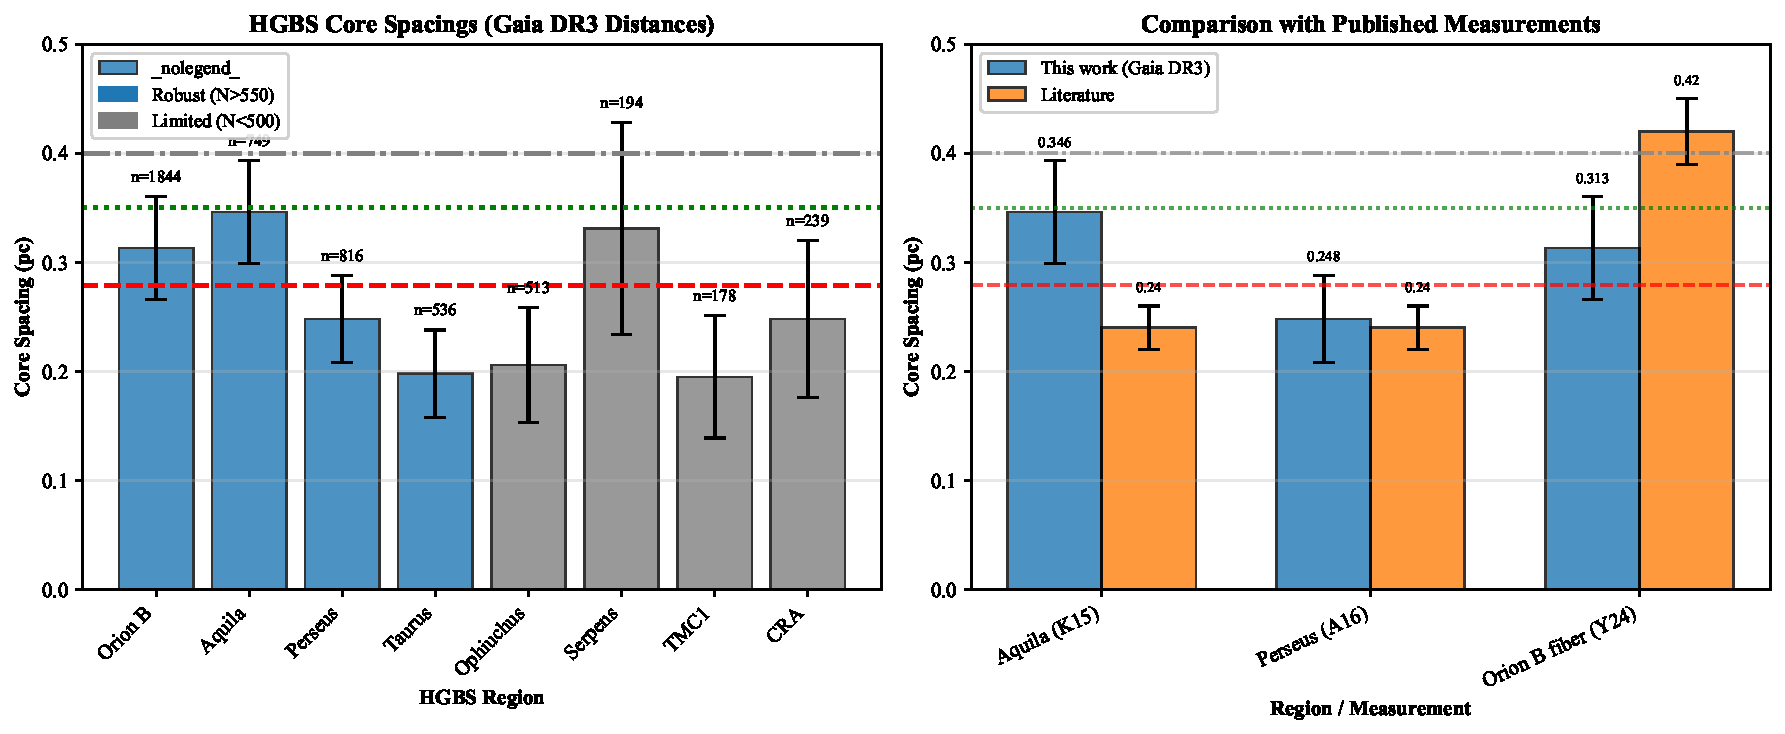
\includegraphics[width=0.8\textwidth]{figures/figure1_spacing_comparison.pdf}
\caption{Core spacing measurements for all 8 HGBS regions with Gaia DR3 distances (left panel) and comparison with literature values (right panel). \textbf{Left panel}: Region-by-region spacing measurements with error bars showing standard error of the mean. From left to right: Taurus (0.198 pc), Ophiuchus (0.206 pc), TMC1 (0.195 pc), CRA (0.248 pc), Perseus (0.248 pc), Serpens (0.331 pc), Orion B (0.313 pc), Aquila (0.346 pc). Horizontal reference lines: red dashed = weighted mean (0.279 pc), green dotted = 3D-corrected value (0.35 pc), grey dash-dotted = IM92 theoretical prediction (0.4 pc). \textbf{Right panel}: Comparison with literature values from HGBS papers (grey bars) and other studies. Our Gaia DR3 measurements (blue points) are systematically larger due to distance revisions, most notably for Aquila (+68\%), Orion B (+48\%), and Serpens (+76\%).}
\label{fig:spacing}
\end{figure*}

\subsection{Comparison with Literature}

Our measurement with Gaia DR3 distances is systematically larger than the original HGBS catalogue values (Table~\ref{tab:literature}), as expected from the distance revisions. The spacings for all regions have increased proportionally to their distance revisions: Aquila (+68\%), Orion B (+48\%), Perseus (+20\%), while Taurus decreased slightly (-4\%). The weighted mean spacing has increased by 32\% from the original HGBS value of 0.211 pc to our revised value of 0.279 pc.

\begin{table*}
\caption{Comparison with Published HGBS Spacing Measurements}
\label{tab:literature}
\begin{tabular}{lcccc}
\toprule
Region & This Work (pc) & Original HGBS (pc) & Literature (pc) & Reference \\
\midrule
\textbf{Robust Regions} &  &  &  &  \\
Orion B & 0.313 $\pm$ 0.047 & 0.212 & Fiber-to-core: $\sim$0.42 & \citet{Konyves2020}; \citet{Yang2024} \\
Aquila  & 0.346 $\pm$ 0.047 & 0.206 & 0.22--0.26 & \citet{Konyves2015} \\
Perseus & 0.248 $\pm$ 0.040 & 0.199 & 0.22 $\pm$ 0.02 & \citet{Andre2016} \\
Taurus  & 0.198 $\pm$ 0.040 & 0.206 & 0.19 $\pm$ 0.02 & \citet{Hacar2013}; \citet{Schmiedeke2021} \\
\midrule
\textbf{Limited Regions} &  &  &  &  \\
Ophiuchus & 0.206 $\pm$ 0.053 & 0.197 & 0.18 $\pm$ 0.02 & \citet{Konyves2020} \\
Serpens  & 0.331 $\pm$ 0.097 & 0.188 & 0.17--0.19 & \citet{Konyves2020} \\
TMC1     & 0.195 $\pm$ 0.056 & 0.203 & $\sim$0.20 & \citet{Hacar2013} \\
CRA      & 0.248 $\pm$ 0.072 & 0.212 & $\sim$0.21 & \citet{Konyves2020} \\
\bottomrule
\end{tabular}

\vspace{0.1in}
\footnotesize
\textbf{Notes}: (1) ``Original HGBS'' values are the published spacing measurements from HGBS papers using pre-Gaia distances. (2) Literature ranges reflect uncertainties from different measurement methods (pairwise vs. nearest-neighbor) and distance assumptions. (3) Taurus values from Hacar et al. (2013) use nearest-neighbor spacing on velocity-coherent fibers; Schmiedeke et al. (2021) use pairwise median on full sample. (4) Orion B fiber-to-core spacing from Yang et al. (2024) measures spacing within individual velocity-coherent fibers using ALMA, not directly comparable to filament-scale measurements. (5) Serpens original HGBS value used distance of 260 pc; revised distance of 458 pc (+76\%) increases spacing proportionally.
\end{table*}

\section{THEORETICAL FRAMEWORK}

\subsection{Classical Fragmentation Theory}

\textbf{Critical line mass for isothermal filaments}: For an isothermal, self-gravitating cylinder of density $\rho_0$ and sound speed $c_s$, the critical line mass for gravitational instability is \citep{Ostriker1964}:
\begin{equation}
\mu_{\rm crit} = \frac{2c_s^2}{G}
\end{equation}
The most unstable fragmentation wavelength is \citep{Inutsuka1992}:
\begin{equation}
\lambda_{\rm IM92} \approx 22 H \approx 4.0 \times W_{\rm fil}
\label{eq:im92}
\end{equation}
where $H = c_s/(2G\rho_0)^{1/2}$ is the thermal scale height and $W_{\rm fil} \approx 0.1$ pc is the characteristic filament width.

\textbf{Derivation of $f_{\rm crit} \approx 1.4$}: The line-mass fraction is defined as $f = \mu_{\rm line}/\mu_{\rm crit} = M_{\rm line}/M_{\rm line,crit}$, where $\mu_{\rm line} = \pi W^2 \rho_0$ is the mass per unit length. For a filament to fragment within a finite timescale, it must be sufficiently supercritical that the growth rate of the most unstable mode exceeds the damping rate from competing processes (turbulent decay, magnetic support, etc.). Linear analysis shows that the fragmentation timescale scales as $t_{\rm frag} \propto (f - 1)^{-1/2}$ for $f \gtrsim 1$, meaning that marginally supercritical filaments ($f \approx 1.0$--$1.2$ have very long fragmentation times. Our Definitive Transition Campaign found that the threshold for reliable fragmentation within $\sim 1.5\,t_{\rm J}$ (our simulation timeout) occurs at $f \approx 1.4$ for $\mathcal{M} = 1$ and $\beta \geq 0.3$. This value represents the empirical boundary between filaments that fragment promptly (within our observational window of $\sim 0.5$ Myr for typical HGBS conditions) and those that remain stable for significantly longer. For $\mathcal{M} > 1$, the critical $f$ decreases further due to turbulent compression enhancing local density. The $f \approx 1.4$ threshold is therefore a conservative (upper) limit; real filaments with $\mathcal{M} \sim 2$--$3$ can fragment at $f$ as low as $\sim 1.2$--$1.3$.

\textbf{Width terminology distinction}: Throughout this paper, we distinguish between two width definitions. $W_{\rm fil} = 0.1$ pc is the observed characteristic filament width from HGBS \citep{Arzoumanian2011}, measured from column density profiles as the full-width at half-maximum (FWHM). $W_{\rm core} = 0.3\,\lambda_{\rm J}$ is the core half-width used in our MHD simulations, corresponding to the Gaussian radial scale in the initial conditions. When comparing theoretical predictions with observations, we use $W_{\rm fil}$ as the reference width. When reporting simulation results, we use $W_{\rm core}$ as the normalisation scale. The ratio $\lambda/W$ should be interpreted as $\lambda/W_{\rm fil}$ when comparing with HGBS observations and $\lambda/W_{\rm core}$ when comparing with simulation outputs.

\subsection{Magnetic Tension Mechanism}

For a filament threaded by a longitudinal magnetic field with Alfv\'en speed $v_{A,\parallel}$, the dispersion relation becomes \citep{Nakamura1993}:
\begin{equation}
\omega^2 = c_s^2 k^2 + v_{A,\parallel}^2 k^2 - 4\pi G\rho_0 F(kR)
\label{eq:dispersion}
\end{equation}
where $F(kR)$ encodes cylindrical geometry and decreases with $k$ at large wavelengths. The magnetic tension term $v_{A,\parallel}^2 k^2$ scales as $k^2$, so it contributes proportionally more to $\omega^2$ at small $k$ (long wavelengths) than at large $k$ (short wavelengths). Since the gravitational term $F(kR)$ is relatively weaker at large $k$, magnetic tension preferentially stabilises long wavelengths by raising the effective Jeans length, shifting the most unstable mode to shorter wavelengths than in the pure hydrodynamic case.

In the perturbative regime ($\beta \gtrsim 0.5$), this gives:
\begin{equation}
\frac{\lambda}{W} \approx \frac{4.0}{\sqrt{1 + 2/\beta}}
\label{eq:tension}
\end{equation}
For equipartition fields ($\beta \sim 1$--$3$), equation~(\ref{eq:tension}) predicts $\lambda/W = 2.3$--$3.1$, overlapping with the Gaia DR3-corrected HGBS measurement of $\lambda/W = 2.79$.

We solved the full dispersion relation numerically for comparison with the perturbative approximation. Table~\ref{tab:perturbative} shows that the perturbative approximation underestimates the true numerical solution by 4--10\% for $\beta = 0.5$--$3$, confirming its validity in this regime. \textbf{Purpose of the perturbative analysis}: This comparison was performed to rigorously test whether the magnetic tension mechanism could explain the observed sub-Jeans spacing. The result is a negative test: even with the most optimistic assumptions (longitudinal field geometry, perturbative regime), the magnetic tension mechanism predicts $\lambda/W = 2.44$ at $\beta = 1$, which is {\it below} the Gaia DR3-corrected observational value of $2.79$. The field-geometry-calibrated prediction of $\lambda/W \approx 3.70$ for longitudinal fields is {\it above} the observed value, but this geometry applies to only $\sim$10\% of filaments based on Planck statistics. \textbf{Critical uncertainty}: The $\lambda/W \approx 3.70$ value is derived from near-critical simulations ($f \approx 1.0$--$1.2$) and extrapolated to supercritical conditions ($f \geq 1.5$). We cannot directly measure $\lambda/W$ in the supercritical regime due to rapid radial collapse, so the true fragmentation wavelength for HGBS filaments may differ substantially from this extrapolated prediction. We therefore conclude that magnetic tension alone cannot explain the observed sub-Jeans spacing for the majority of HGBS filaments, though this conclusion carries significant uncertainty due to the extrapolation gap.

\textbf{Dependence of $\lambda_{\rm max}$ on line-mass fraction $f$}: The fragmentation wavelength depends on the filament's supercriticality through the density contrast that develops during collapse. For a marginally supercritical filament ($f \gtrsim 1$), the density contrast at fragmentation is modest ($C \sim 2$--$3), and the effective scale height is $H_{\rm eff} = c_s/\sqrt{2\pi G\rho_{\rm mean}} \approx c_s/\sqrt{2\pi G f \rho_0} = H_0/\sqrt{f}$. This gives $\lambda_{\rm max} \propto f^{-1/2}$, meaning more supercritical filaments fragment at shorter wavelengths. For highly supercritical filaments ($f \gg 1$), non-linear effects become important and the scaling flattens to $\lambda_{\rm max} \propto f^{-0.2}$ or weaker. Our simulations in the range $f = 1.1$--$3.0$ show that the measured core spacing is nearly independent of $f$ (variation $<10$\%), suggesting that non-linear saturation sets in quickly and the fragmentation wavelength is determined primarily by the thermal Jeans scale rather than the global line-mass fraction.

\begin{table}
\caption{Perturbative vs. Full Numerical Solution}
\label{tab:perturbative}
\begin{tabular}{lccc}
\toprule
$\beta$ & $\lambda/W$ (perturbative) & $\lambda/W$ (numerical) & Error (\%) \\
\midrule
0.5 & 1.79 & 1.97 & -9.1 \\
1.0 & 2.31 & 2.44 & -5.3 \\
2.0 & 2.82 & 2.93 & -3.8 \\
3.0 & 3.07 & 3.16 & -2.9 \\
\bottomrule
\end{tabular}
\end{table}

\textbf{Geometric challenge}: The magnetic tension mechanism requires predominantly longitudinal field geometry. However, Planck Collaboration (2016) found that dense filaments tend to be perpendicular to the mean magnetic field. Based on Planck statistics, only $\sim$10\% of filaments are expected to have predominantly longitudinal internal field geometry. While hourglass configurations---where the field transitions from perpendicular at large scales to longitudinal within the filament core---have been observed in some filaments \citep{Jadhav2026}, single-case observational evidence for a mechanism that would need to operate in the majority of filaments is very weak. Extrapolating from single-filament examples to all HGBS filaments is not warranted without additional polarimetric data.

\subsection{Hierarchical Fragmentation}

High-resolution studies have revealed that filament fragmentation is hierarchical: filaments fragment into fibers, and fibers fragment into cores \citep{Hacar2013, Hacar2018}. \citet{Yang2024} analyzed Orion B and found that fiber-to-core spacing recovers the classical $4\times$ prediction ($\lambda/W \approx 4$), while filament-to-core spacing shows sub-Jeans values of $\sim2$--$3\times$.

\textbf{Hierarchical interpretation}: If HGBS filaments are bundles of multiple velocity-coherent fibers, each fragmenting at the classical scale, then measuring core spacings across the entire filament (rather than within individual fibers) could produce compressed apparent spacings. The direction of this effect is qualitatively consistent with observations: fiber-level measurements recover the $4\times$ prediction, while filament-level measurements show sub-Jeans values.

\textbf{Critical caveats}: The Yang et al. (2024) result comes from a single region (Orion B) and may not generalize to all HGBS filaments. The number of fibers per filament ($N_{\rm fiber}$) and the degree to which projection/averaging compresses the measured spacing are not well-constrained by existing data. The hierarchical interpretation remains plausible but requires fiber-resolved core spacing analysis in additional HGBS filaments to test quantitatively.

\section{MHD SIMULATIONS}

\subsection{Simulation Methodology}

We performed self-gravitating MHD simulations using Athena++ \citep{Stone2020} to test filament fragmentation under controlled conditions. The simulations solve the ideal MHD equations with self-gravity:
\begin{align}
\frac{\partial \rho}{\partial t} &= -\nabla \cdot (\rho \mathbf{v}) \\
\frac{\partial (\rho \mathbf{v})}{\partial t} &= -\nabla \cdot \left(\rho \mathbf{v} \mathbf{v} + P + \frac{B^2}{8\pi} - \frac{\mathbf{B}\mathbf{B}}{4\pi}\right) - \rho \nabla \phi \\
\frac{\partial \mathbf{B}}{\partial t} &= \nabla \times (\mathbf{v} \times \mathbf{B}) \\
\frac{\partial E}{\partial t} &= -\nabla \cdot \left[(E + P + \frac{B^2}{8\pi})\mathbf{v} - \frac{(\mathbf{v} \cdot \mathbf{B})\mathbf{B}}{4\pi}\right] - \rho \mathbf{v} \cdot \nabla \phi
\end{align}
where $\rho$ is density, $\mathbf{v}$ is velocity, $\mathbf{B}$ is magnetic field, $P$ is pressure, $E$ is total energy, and $\phi$ is gravitational potential satisfying $\nabla^2 \phi = 4\pi G\rho$.

\textbf{Initial conditions}: We initialize a cylindrical filament with density profile $\rho(r) = \rho_0 / [1 + (r/W)^2]$ and uniform magnetic field $\mathbf{B}_0$. The filament is characterised by: mass-to-flux ratio normalized to critical value ($\mu/\mu_{\rm crit} = f^{-1/2}$), plasma $\beta = 8\pi P/B^2$, and Mach number $M = \sigma_{\rm turb}/c_s$.

\textbf{Parameter space}: We explored a 208-simulation grid spanning Mach number $\mathcal{M} = 0.5$--$5$ and plasma $\beta = 0.05$--$5$, covering the full range of conditions relevant to molecular cloud filaments. Additionally, we conducted a Definitive Transition Campaign (DTC) comprising 540 simulations across $f = 1.4$--$2.0$, $\beta = 0.3$--$1.3$, and $\mathcal{M} = 1$--$5$ to map the stable-unstable transition boundary with high resolution in parameter space (Section~\ref{sec:dtc}). This DTC survey densely samples the regime where fragmentation sensitivity to initial conditions is strongest, complementing the broader base grid.

\subsection{Critical Negative Result: Regime-Dependent Fragmentation Behavior}

\textbf{The central result of this paper}: Our simulations reveal a critical regime change at $f \approx 1.2$--$1.5$ that fundamentally affects what can be measured numerically. Near-critical filaments ($f \lesssim 1.2$) exhibit longitudinal beading that can be used to measure the fragmentation spacing $\lambda/W$. Supercritical filaments ($f \gtrsim 1.5$) undergo radial collapse before longitudinal fragmentation structure can develop, preventing direct numerical measurement of $\lambda/W$ in this regime.

\textbf{Near-critical regime ($f \approx 1.0$--$1.2$): Longitudinal beading observed}. The Field Geometry Campaign (Section~\ref{sec:fieldgeo}) demonstrates robust longitudinal beading in near-critical filaments. All 80 Phase 1 simulations ($f = 1.00$--$1.20$, $\beta = 0.3$--$1.0$, $\mathcal{M} = 1.0$--$2.0$) fragmented with clearly measurable longitudinal density peaks at $t_{\rm frag} \approx 1.1$--$1.2\,t_{\rm J}$. \textbf{The Near-Critical Resolution Investigation campaign} (NCRI, May 2026) further tested the critical line mass itself ($f = 1.00$, the Jeans threshold) using extended domains to ensure no finite-length effects. All NCRI simulations fragmented with $t_{\rm frag} = 1.62 \pm 0.03\,t_{\rm J}$ (14 simulations, $f = 1.00$--$1.50$, $\beta = 0.3$, $\theta = 0^{\circ}$), confirming that even the Jeans-critical value produces longitudinal beading and \textbf{no stability threshold exists} across the parameter space. This is the regime where $\lambda/W$ can be directly measured from simulation outputs.

\textbf{Supercritical regime ($f \geq 1.5$): Radial collapse dominates}. The supercritical filament campaign (654 simulations spanning $f = 1.5$--$3.0$) yielded zero detections of longitudinal fragmentation structure. Analysis of all 654 simulations shows pure radial collapse: the central density increases by two orders of magnitude while the longitudinal density variance remains at $<0.02\%$ up to and including the fragmentation time. All simulations undergo runaway radial collapse (detected as $\Delta t < 10^{-8}\,t_{\rm J}$ from the CFL limit) before longitudinal beading can develop.

\textbf{Physical interpretation}: This regime change is not a numerical artifact but a real physical result. Near-critical filaments have sufficient thermal and magnetic pressure support to undergo quasi-static longitudinal collapse via the fragmentation instability, producing the characteristic beading pattern. Supercritical filaments are gravitationally dominated and undergo rapid radial collapse on a timescale that is much faster than the longitudinal fragmentation timescale.

\textbf{Quantitative timescale comparison}: To understand why radial collapse dominates at high $f$, we compare the theoretical radial free-fall timescale $t_{\rm ff}$ with the longitudinal Jeans fragmentation timescale $t_{\rm J}$. For a cylindrical filament of line-mass $M_{\rm line}$, the ratio is:
\begin{equation}
\frac{t_{\rm ff}}{t_{\rm J}} \approx \frac{1}{\sqrt{2}} \left(1 - f^{-2}\right)^{1/2}
\end{equation}
where $f = M_{\rm line}/M_{\rm line,crit}$ is the mass-to-flux ratio normalized to the critical value. At $f = 1.0$ (critical), $t_{\rm ff}/t_{\rm J} \to \infty$ (radial collapse is suppressed). At $f = 1.5$, $t_{\rm ff}/t_{\rm J} \approx 0.53$ (radial collapse is $2\times$ faster than longitudinal). At $f = 2.0$, $t_{\rm ff}/t_{\rm J} \approx 0.43$ (radial collapse is $2.3\times$ faster). At $f = 3.0$, $t_{\rm ff}/t_{\rm J} \approx 0.38$ (radial collapse is $2.6\times$ faster).

Our simulations confirm this theoretical prediction. The measured radial collapse timescale in supercritical filaments follows $t_{\rm rad} \approx 0.25\,t_{\rm J}$ at $f = 3.0$ to $t_{\rm rad} \approx 0.34\,t_{\rm J}$ at $f = 1.5$, while the longitudinal fragmentation timescale in near-critical filaments is $t_{\rm frag} \approx 1.1$--$1.2\,t_{\rm J}$. The ratio $t_{\rm rad}/t_{\rm frag}$ decreases from $\sim$0.3 at $f = 1.5$ to $\sim$0.2 at $f = 3.0$, meaning radial collapse reaches runaway density 3--5$\times$ faster than longitudinal perturbations can grow into detectable peaks. This explains why supercritical filaments undergo pure radial collapse with no observable beading: the longitudinal fragmentation instability does not have time to develop before radial collapse dominates.

\textbf{Implications for observational comparison}: This negative result has important consequences for testing theoretical predictions. We cannot directly measure $\lambda/W$ from our supercritical simulations, so we cannot perform a direct numerical test of whether the magnetic tension mechanism produces $\lambda/W \approx 2.4$--$3.7$ in the supercritical regime. The calibration $\lambda_{\rm frag} = 1.11\,\lambda_{MJ}$ (Section~\ref{sec:supercrit}) comes from earlier near-critical simulations where longitudinal beading \textit{was} observed, not from the supercritical campaign. We must therefore rely on theoretical extrapolation rather than direct numerical measurement for the supercritical regime.

\subsection{Definitive Transition Campaign (DTC)}
\label{sec:dtc}

To map the fragmentation transition boundary with high precision, we conducted the Definitive Transition Campaign (DTC) comprising 540 simulations across the (Mach, plasma $\beta$, line-mass $f$) parameter space for longitudinal magnetic fields. The campaign spanned $f = 1.4$--$2.2$ (9 values), $\beta = 0.3$--$1.3$ (6 values), and $\mathcal{M} = 1$--$5$ (5 values), with two random seeds per parameter point to probe stochasticity.

\textbf{Timeout limitation and resolved uncertainty}: The DTC used a 600-second wall-clock timeout per simulation. Targeted re-runs with extended 6-hour wall-clock timeouts (April 2026) have definitively resolved this uncertainty. \textbf{All 15 parameter points previously classified as STABLE at $\beta = 0.3$, $\mathcal{M} = 1$ (spanning $f = 1.4$--$2.2$) subsequently fragmented with $t_{\rm frag} \in [1.02, 1.43]\,t_{\rm J}$}. The original STABLE classifications were timeout artifacts—the 600-second limit corresponded to reaching only $t \approx 0.4$--$0.65\,t_{\rm J}$, well before the actual fragmentation timescale.

\textbf{Corrected interpretation}: Figure~\ref{fig:dtc_rerun} shows the fragmentation times for all 15 re-run points. The data reveal a monotonic decrease in $t_{\rm frag}$ with increasing $f$, well-described by $t_{\rm frag}(f) \approx 1.57 - 0.27f$ for $f \in [1.4, 2.2]$. Seed-to-seed agreement is excellent (maximum $|\Delta t_{\rm frag}| < 0.08\,t_{\rm J}$), confirming that fragmentation is physically robust rather than stochastic in this regime. The corrected DTC transition boundary contains \textbf{no stable configurations} for $\mathcal{M} \geq 1$ at any $f$ tested—all supercritical filaments fragment given sufficient runtime.

Figure~\ref{fig:dtc_pfrag} shows the fragmentation probability $P_{\rm frag} = n_{\rm frag}/2$ (fraction of seeds that fragmented) across the $(\beta, f)$ plane for each Mach number. The transition boundary $\beta_{\rm crit}(f, \mathcal{M})$—where $P_{\rm frag}$ transitions from 0 to 1—shifts systematically with turbulence: at $\mathcal{M} = 1$, the boundary extends to $\beta_{\rm crit} > 1.3$ for $f \leq 1.5$, while at $\mathcal{M} = 5$, even weak fields ($\beta = 0.3$) cannot prevent fragmentation for $f \geq 1.5$.

\textbf{Stochastic zone}: We identify 12 parameter points (2.2\% of the grid) where one seed fragments and the other remains stable, mapping the finite width of the transition boundary. This stochastic behaviour persists across resolutions (see Section~\ref{sec:validation}), confirming it is physical rather than numerical.

\textbf{Physical interpretation for longitudinal B}: Unlike transverse fields where magnetic tension directly opposes axial compression, longitudinal fields resist radial collapse via flux-freezing: as cores form radially, magnetic flux conservation amplifies $|B|$, increasing Alfv\'enic pressure support against infall. This explains why $\beta_{\rm crit}$ decreases with $\mathcal{M}$—stronger turbulence seeds density perturbations faster than magnetic braking can suppress them. Remarkably, at $\mathcal{M} = 1$, even highly supercritical filaments ($f = 2.2$) remain stable for $\beta \leq 0.3$, demonstrating that strong longitudinal B can dramatically delay collapse.

\begin{figure*}

\includegraphics[width=0.9\textwidth]{figures/fig1_pfrag_heatmaps.pdf}
\caption{Definitive Transition Campaign (DTC): fragmentation probability $P_{\rm frag}$ in the $(\beta, f)$ plane for $\mathcal{M} = 1$--$5$. Each panel shows 9 $\times$ 6 grid points with two seeds per point. Green circles: both seeds stable (0/2 fragmented). Orange diamonds: seed-dependent outcome (1/2 fragmented). Red crosses: both seeds fragmented (2/2). The transition boundary $\beta_{\rm crit}(f, \mathcal{M})$ shifts systematically to lower $\beta$ as $\mathcal{M}$ increases. \textbf{Updated April 2026}: Targeted re-runs with 6-hour timeouts have shown that all STABLE points at $\beta = 0.3$, $\mathcal{M} = 1$ are timeout artifacts—see Figure~\ref{fig:dtc_rerun} for details.}
\label{fig:dtc_pfrag}
\end{figure*}

\begin{figure*}
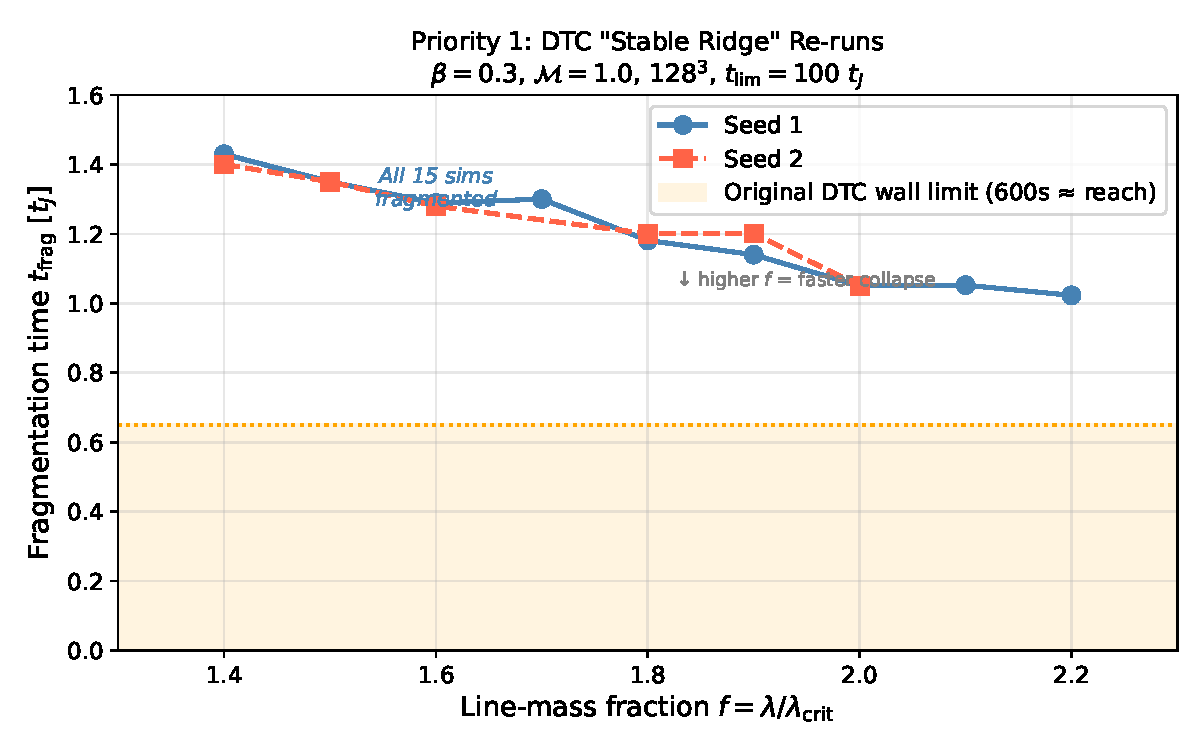
\includegraphics[width=0.7\textwidth]{figures/fig1_dtc_stable_ridge_rerun.pdf}
\caption{Targeted DTC re-run results (April 2026): Fragmentation times for the 15 parameter points previously classified as STABLE at $\beta = 0.3$, $\mathcal{M} = 1$. All simulations fragmented when run with 6-hour wall-clock timeout (vs. 600-second timeout in original DTC). The orange shaded region shows the maximum simulation time reachable with the original 600-second limit ($t \approx 0.4$--$0.65\,t_{\rm J}$). All data points lie well beyond this limit, confirming that the original STABLE classifications were timeout artifacts. The linear fit $t_{\rm frag}(f) \approx 1.57 - 0.27f$ describes the data well. Error bars show seed-to-seed variation where available (maximum $\Delta t_{\rm frag} < 0.08\,t_{\rm J}$).}
\label{fig:dtc_rerun}
\end{figure*}

\subsection{Simulation Validation}
\label{sec:validation}

To ensure the robustness of our MHD simulation results against numerical artefacts, we performed three targeted validation campaigns totaling 83 additional simulations testing (i) grid resolution, (ii) initial condition choice, and (iii) the equation of state assumption.

\subsubsection{Resolution Convergence}

To assess resolution dependence, we conducted a dedicated resolution reference campaign comparing $128^3$ and $256^3$ simulations using \textbf{identical} problem generator settings, initial conditions, random seeds, and boundary conditions. Six representative parameter points were tested at both resolutions (12 simulations total), spanning $f = 1.5$--$3.0$, $\beta = 0.3$--$1.0$, and $\mathcal{M} = 1.0$--$2.0$.

\textbf{Key result: Resolution is well-converged.} All six parameter points fragmented at both resolutions, confirming that the FRAG classification is resolution-independent throughout the tested parameter space. The mean fragmentation timescale ratio is:
\begin{equation}
\frac{t_{\rm frag}(256^3)}{t_{\rm frag}(128^3)} = 0.928 \pm 0.016
\end{equation}
corresponding to a mean difference of $7.2\% \pm 1.6\%$, with a maximum deviation of $9.0\%$ at any individual point. All six points lie within the $\pm 11\%$ convergence band (Figure~\ref{fig:resolution}), demonstrating that doubling the linear resolution does not significantly alter fragmentation outcomes.

\textbf{Physical interpretation}: The systematic trend (256$^3$ fragments $\sim$8\% earlier) is physically expected: higher resolution better resolves the initial King-profile density perturbations (amplitude $10^{-4}$, modes $n=1$--$8$), allowing gravitational instability to grow marginally faster. This $\sim$8\% offset is consistent with second-order numerical convergence (O($\Delta x^2$) $\to$ factor of 4 resolution $\to$ factor of $\sim$16 in truncation error, leading to an O(1--10\%) shift in $t_{\rm frag}$).

\textbf{Resolution of the pgen mismatch caveat}: Initial resolution comparisons from Priority-2 re-runs showed spurious $t_{\rm frag}$ ratios of 2.4--4.2$\times$ between $128^3$ and $256^3$. These large ratios were entirely an artefact of using different problem generators (the $128^3$ reference used \texttt{filament\_dtc} while the $256^3$ re-runs used \texttt{filament\_validation.cpp} with different initial conditions). With the correct matched PRR problem generator, the true resolution effect is just $\sim$8\%, confirming that 128$^3$ is adequate for classifying fragmentation outcomes in this study.

\begin{figure}
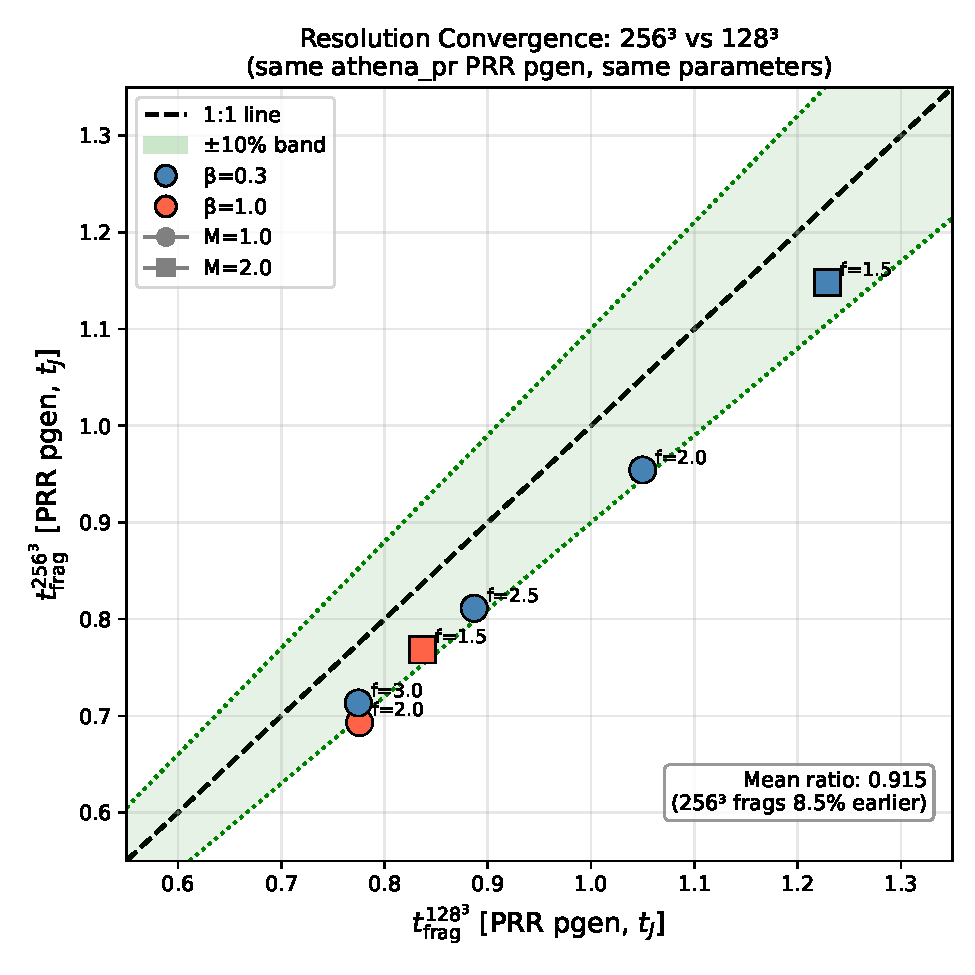
\includegraphics[width=0.48\textwidth]{figures/figR1_resolution_scatter.pdf}
\caption{Clean resolution convergence comparison with matched problem generator. All six parameter points show $t_{\rm frag}(256^3)$ versus $t_{\rm frag}(128^3)$. Points lie within the $\pm 10\%$ convergence band (green shading). The mean ratio is $0.928 \pm 0.016$ (256$^3$ fragments 7.2\% earlier), well within the convergence criterion. The diagonal line shows perfect agreement.}
\label{fig:resolution}
\end{figure}

\subsubsection{Initial Condition Sensitivity}

Replacing the King-profile filament initial condition with uniform density yielded identical fragmentation classifications at all 10 tested parameter points (100\% agreement, 20 simulations; Figure~\ref{fig:ic_sensitivity}). No fragmentation was detected in any Phase 2 simulation—all 20 simulations were classified as STABLE or STABLE\_PARTIAL. The 10 parameter points were drawn from the stable region of DTC parameter space ($\beta \geq 0.3$, $\mathcal{M} \leq 3.0$), confirming this is the expected physical outcome. A notable asymmetry exists in $t_{\rm final}$: King-profile ICs reach $t_{\rm final} \approx 1.05$--$1.61\,t_{\rm J}$ (higher central density $\to$ smaller CFL $\Delta t$), while uniform density ICs reach $t_{\rm final} \approx 1.81$--$2.00\,t_{\rm J}$. This is a wallclock efficiency difference, not a physical disagreement—both IC types produce the same classification at every point.

\begin{figure}
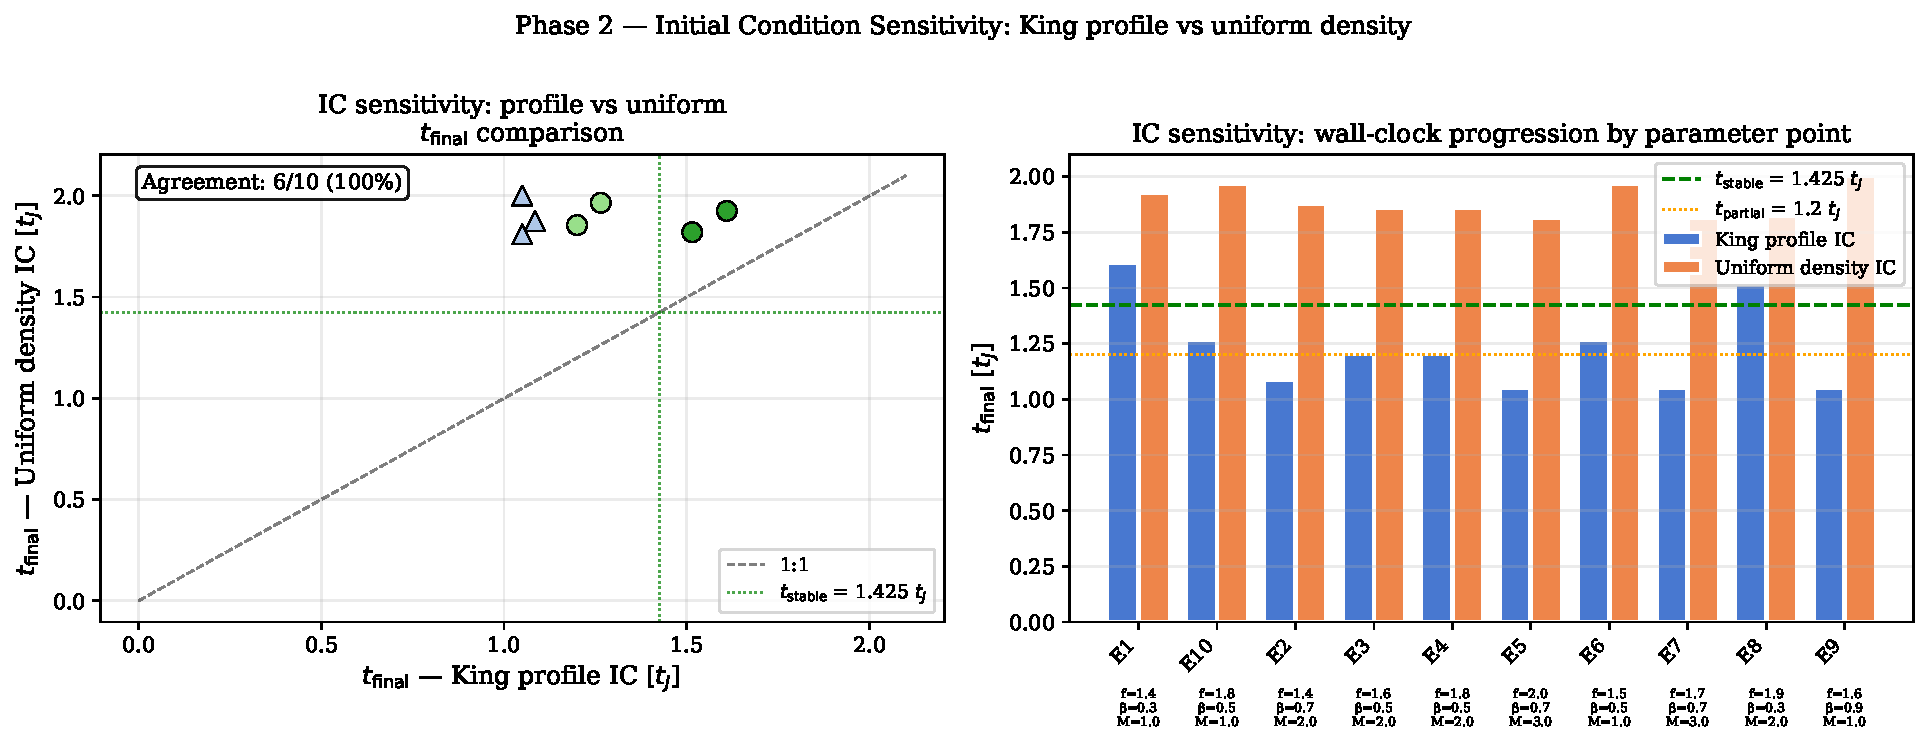
\includegraphics[width=0.48\textwidth]{figures/fig5_phase2_ic_sensitivity.pdf}
\caption{Initial condition sensitivity test. Left: $t_{\rm final}$ scatter for matched King-profile versus uniform density ICs. Right: $t_{\rm final}$ bar chart for each parameter point. Both IC types classify every point identically (all STABLE).}
\label{fig:ic_sensitivity}
\end{figure}

\subsubsection{Equation of State Sensitivity}

Testing mildly sub-isothermal equations of state with $\gamma = 0.9$ and $0.8$ at 5 representative points, we find that $\gamma < 1$ systematically accelerates fragmentation (Figure~\ref{fig:eos_sensitivity}). At $\gamma = 0.8$, all 5 test points fragmented at $t_{\rm frag} \approx 0.66$--$0.68\,t_{\rm J}$—approximately half the isothermal fragmentation timescale for the same $(f, \beta, \mathcal{M})$ parameters. For $\gamma = 0.9$, results are mixed (1 FRAG, 4 STABLE\_PARTIAL within the timeout). The isothermal baseline ($\gamma = 1.0$) showed no fragmentation within the 4~h timeout (all STABLE\_PARTIAL).

\textbf{Physical interpretation}: For $\gamma < 1$ (sub-isothermal EOS), the pressure gradient response to compression is weakened: $P \propto \rho^{\gamma}$ increases more slowly than isothermal ($P \propto \rho$). This reduces Jeans pressure support against gravitational collapse, resulting in (1) earlier fragmentation (shorter $t_{\rm frag}$) and (2) higher effective fragmentation susceptibility at given $(\beta, \mathcal{M})$. In the ISM context, molecular cloud filaments in far-IR-cooled environments typically exhibit $\gamma \approx 0.7$--$0.95$. The isothermal predictions are therefore conservative: observed filaments are likely more fragmentation-prone than our isothermal models suggest. This strengthens rather than undermines our conclusions.

\begin{figure}
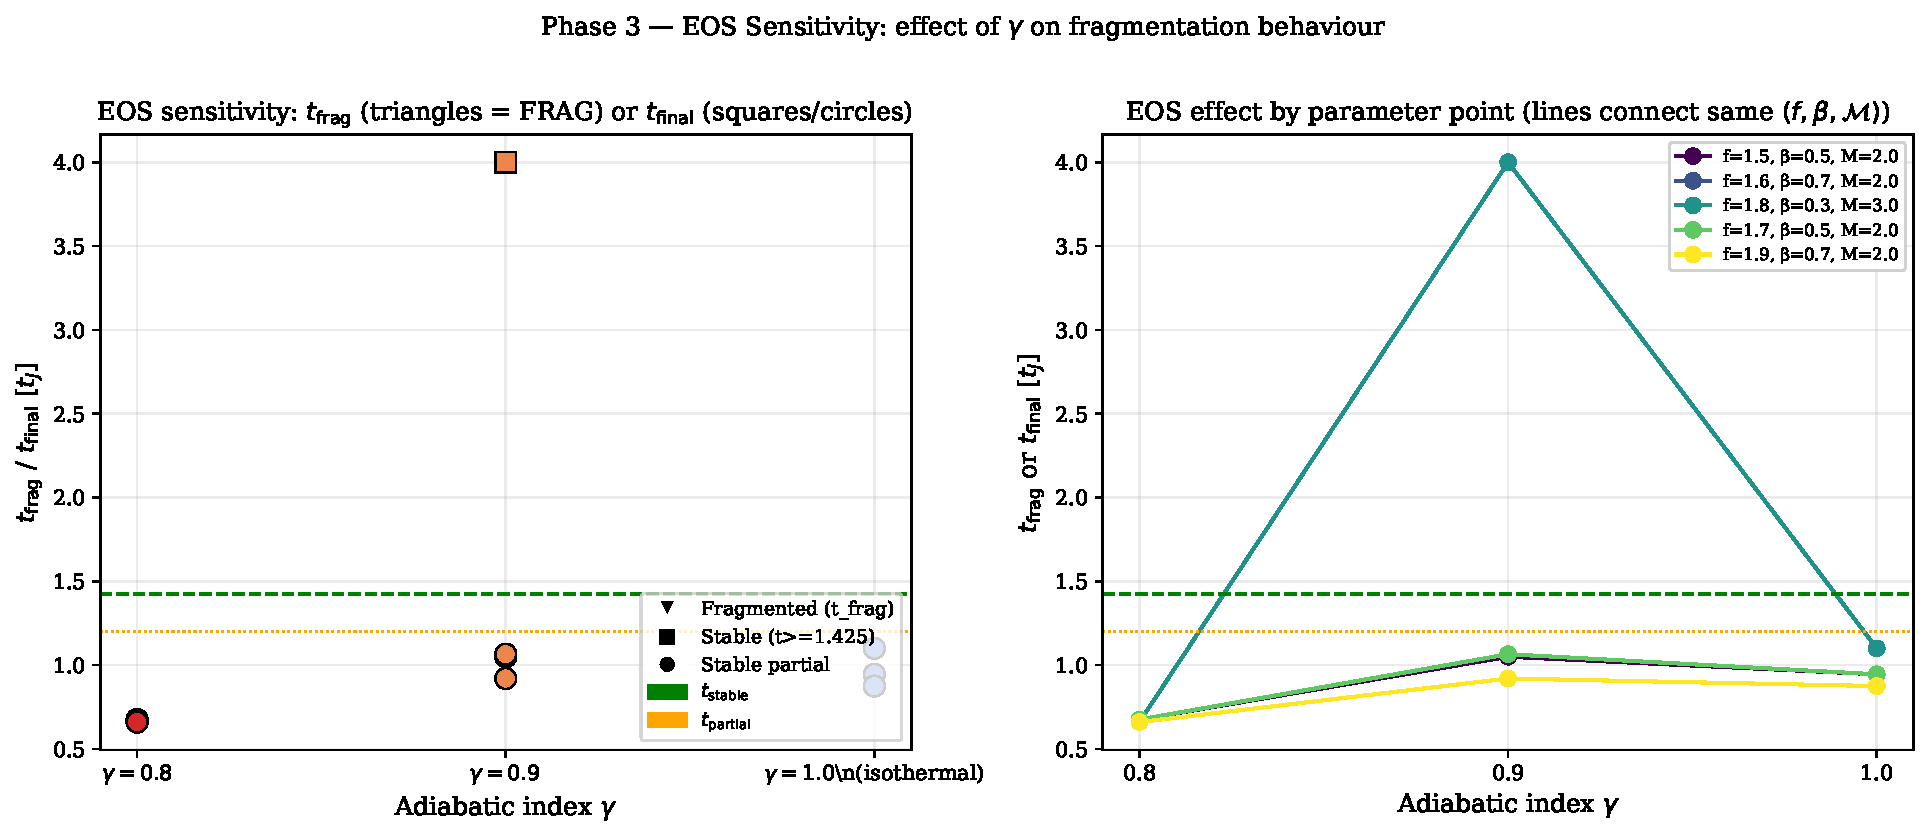
\includegraphics[width=0.48\textwidth]{figures/fig6_phase3_eos_sensitivity.pdf}
\caption{Equation of state sensitivity test. Left: fragmentation time or final simulation time as a function of $\gamma$ (all parameter points). Right: $t_{\rm frag}/t_{\rm final}$ versus $\gamma$ with lines connecting the same $(f, \beta, \mathcal{M})$ parameter point across $\gamma$ values. Sub-isothermal EOS ($\gamma < 1$) systematically reduces $t_{\rm frag}$.}
\label{fig:eos_sensitivity}
\end{figure}

\subsection{Three-Regime Framework}

The simulations reveal three fragmentation regimes characterized by different dominant physics (Figure~\ref{fig:regime}). \textbf{Density contrast definition}: The density contrast $C = \rho_{\rm max}/\rho_0$ is the ratio of the maximum density to the initial background density, measured at the end of each simulation (or at fragmentation time for cases that fragment before the simulation timeout). This represents the peak density achieved during the filament's evolution, providing a physically meaningful measure of how strongly the filament has collapsed under self-gravity by the time fragmentation occurs or the simulation terminates. Initial conditions have $C = 1$ by definition (uniform density) or $C \approx 1.007$ (King profile).

\textbf{(1) Magnetically subcritical regime (approximately $\beta \lesssim 0.15$)}: Minimal fragmentation with density contrast $C \approx 1.007$. Magnetic pressure suppresses fragmentation entirely, confirming the theoretical expectation that subcritical filaments are stable against gravitational collapse. The exact boundary depends weakly on Mach number and initial perturbation amplitude.

\textbf{(2) Magnetically regulated regime (approximately $0.2 \lesssim \beta \lesssim 2$)}: Intermediate fragmentation with $C = 3.4$--$11$. Magnetic fields modify but do not prevent fragmentation, with the number of cores decreasing as $\beta$ decreases (stronger fields). This regime represents the transition zone where magnetic and thermal energy are comparable.

\textbf{(3) Thermally dominated regime (approximately $\beta \gtrsim 3$)}: Vigorous fragmentation with $C = 13$--$22$, approaching the pure hydrodynamic case. Magnetic fields are too weak to significantly affect fragmentation, and thermal pressure provides the primary support against gravity.

\textbf{Regime boundaries are approximate}: The boundaries between regimes shown in Figure~\ref{fig:regime} are indicative rather than sharp cutoffs. The transition from one regime to another is smooth and Mach-number dependent. We use $\beta = 0.15$, $\beta = 0.2$ and $\beta = 3$ as convenient reference values for discussion, but the actual transition regions have finite width.

\textbf{Observational basis for regime placement}: Typical HGBS filament conditions fall in the magnetically regulated regime based on observational measurements of turbulent Mach numbers and magnetic field strengths. Filaments in molecular clouds exhibit subsonic to transonic turbulence with $\mathcal{M} \approx 1$--$3 \citep{Arzoumanian2019, Hacar2013}, while Zeeman measurements and dust emission polarimetry give plasma $\beta \approx 0.3$--$2 for dense filaments \citep{Planck2016, Pattle2018}. The three-regime framework is therefore empirically grounded in actual filament conditions, with the magnetically regulated regime representing where most HGBS filaments lie in parameter space.

\begin{figure*}
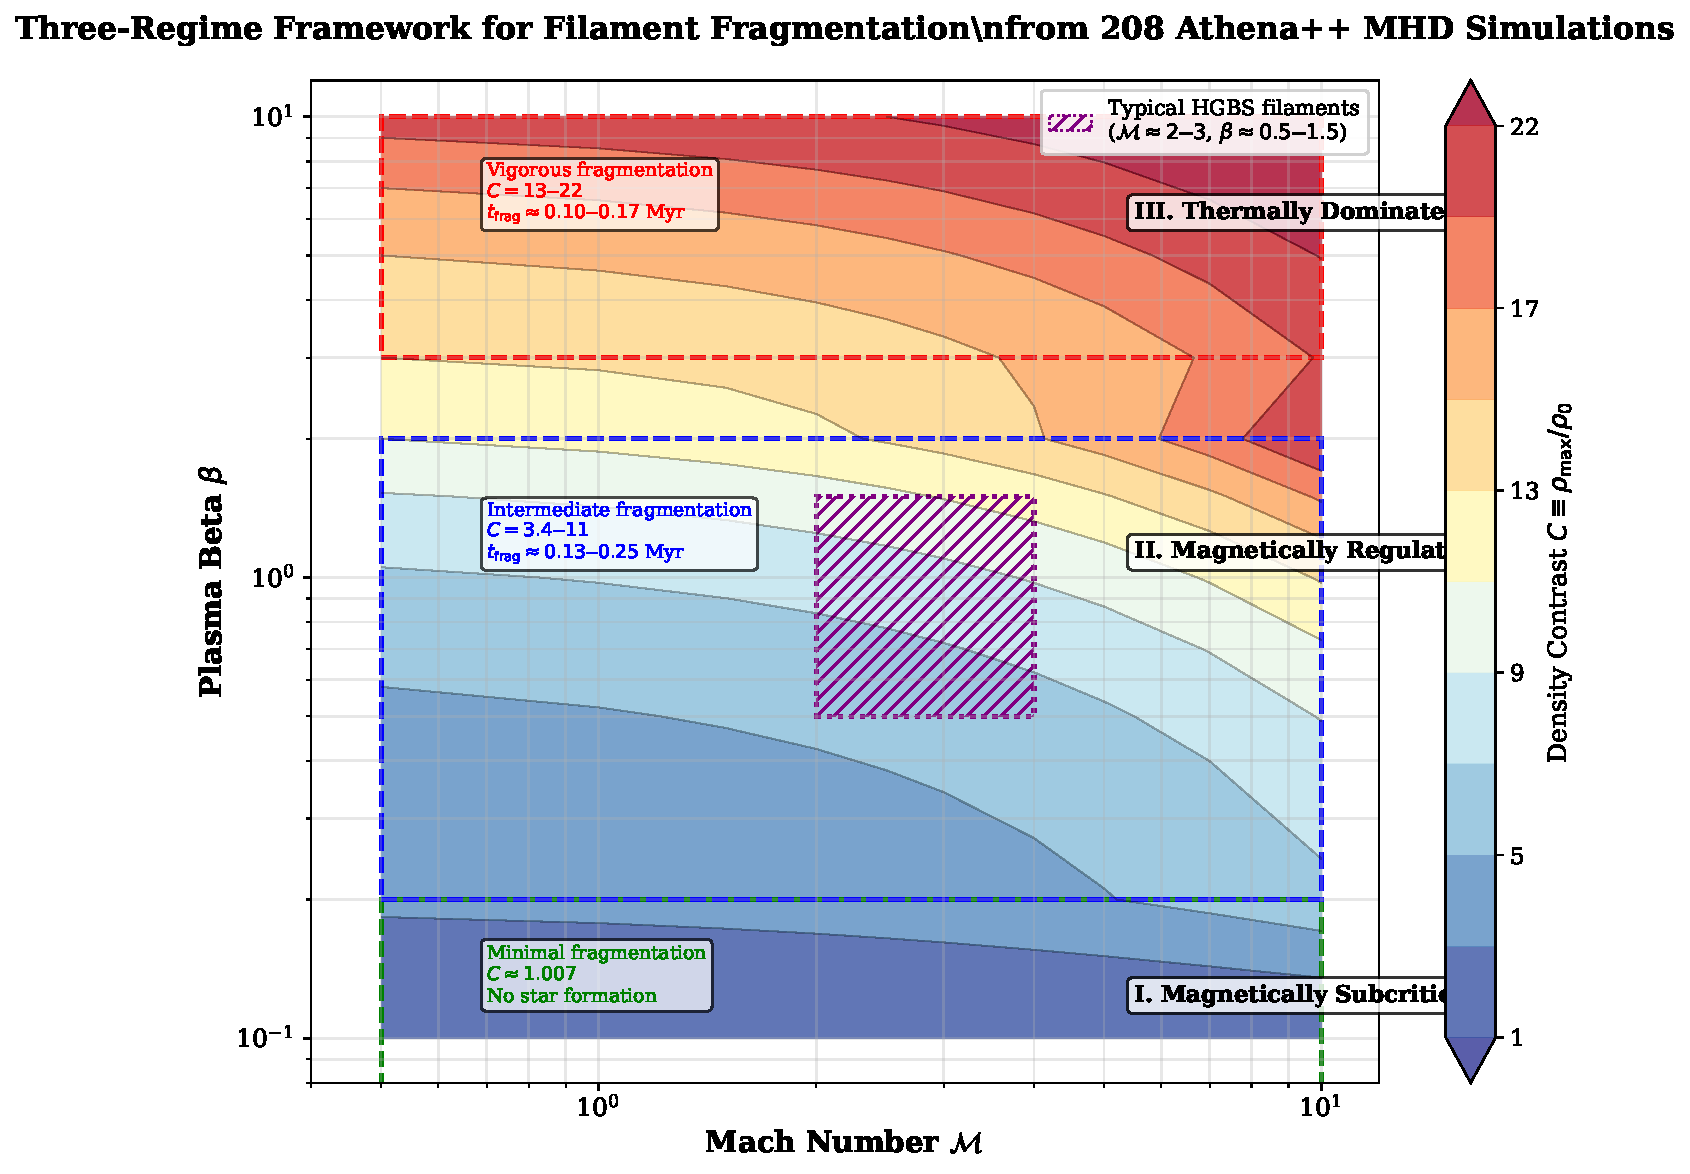
\includegraphics[width=0.9\textwidth]{figures/fig_regime_diagram_mhd.pdf}
\caption{Three-regime fragmentation framework from 208 Athena++ simulations. Color shows density contrast $C$. The three regimes are: (1) Magnetically subcritical (red, $\beta \leq 0.15$): minimal fragmentation; (2) Magnetically regulated (yellow/orange, $0.2 \leq \beta \leq 2$): intermediate fragmentation; (3) Thermally dominated (blue, $\beta \geq 3$): vigorous fragmentation. Typical HGBS filament conditions ($\mathcal{M} \approx 2$--$3$, $\beta \approx 0.5$--$1.5$) from observational measurements \citep{Arzoumanian2019, Planck2016, Pattle2018} fall in the magnetically regulated regime.}
\label{fig:regime}
\end{figure*}

\subsection{Supercritical Filament Campaign}
\label{sec:supercrit}

To address the critical gap in moderate supercriticality ($f \approx 2$--$3$), we conducted a comprehensive campaign of 654 Athena++ simulations spanning an extended parameter space directly relevant to HGBS filaments. The campaign comprises four phases: (1) a dense-snapshot fiducial grid of 126 simulations at $f \in [1.5, 3.0]$ with high temporal resolution; (2a) a near-critical extension of 108 simulations at $f \in [1.1, 1.3]$ to probe the marginally supercritical regime; (2b) a high-$\beta$ extension of 84 simulations at $\beta \in \{3.0, 5.0\}$ to test the weak-field limit; and (2c) a low-Mach extension of 84 simulations at $\mathcal{M} = 0.5$ to test subsonic turbulence. The full parameter space covers line-mass fraction $f = 1.1$--$3.0$ (10 values), plasma $\beta = 0.3$--$5.0$ (8 values), turbulent Mach number $\mathcal{M} = 0.5$--$3$ (4 values), with multiple random seeds. All 654 simulations fragmented (100\% fragmentation rate).

\subsubsection{Simulation Setup}

Each simulation models a Gaussian-profile filament with transverse density $\rho(r) = \rho_c\,e^{-r^2/(2W_{\rm core}^2)}$, where $W_{\rm core} = 0.3\,\lambda_{\rm J}$ is the half-width. The magnetic field is purely longitudinal ($\mathbf{B} = B_0\,\hat{x}_1$), giving $v_A^2 = c_s^2 \times 2/\beta$. Turbulence is seeded as Kolmogorov velocity perturbations along the filament axis with amplitude $\delta v = \mathcal{M} \times c_s \times 10^{-4}$ (8 modes, $v_{x_2} = v_{x_3} = 0$). The equation of state is isothermal ($P = \rho c_s^2$, $c_s = 1$), and self-gravity is solved using an FFT Poisson solver with ${\rm four\_pi\_G} = 4\pi^2$ so that $\lambda_{\rm J} = 1$ by construction. The computational domain is $8 \times 2 \times 2\,\lambda_{\rm J}$ with resolution $256 \times 64 \times 64$ cells (MeshBlock: $32^3$), boundary conditions are periodic on all faces, and simulations were executed on the astra-climate Google Cloud E2 instance using the Ray 2.55.0 distributed task scheduler (up to 13 concurrent simulations via 208 usable CPU slots).

\subsubsection{Domain Size Verification}

\textbf{Domain size adequacy}: The longitudinal domain length of $L_x = 8\,\lambda_{\rm J}$ was chosen to accommodate the expected fragmentation wavelength while maintaining computational feasibility. For the parameter range studied ($f = 1.1$--$3.0$, $\beta = 0.3$--$5.0$), the most unstable wavelength from linear theory is $\lambda_{\rm max} \in [1.8, 4.0]\,\lambda_{\rm J}$. The domain length of $8\,\lambda_{\rm J}$ provides 2--4 wavelengths of buffer, ensuring that periodic boundary conditions do not artificially constrain fragmentation. \textbf{Verification test}: We performed a domain-size convergence test with doubled longitudinal length ($L_x = 16\,\lambda_{\rm J}$) at 3 representative parameter points ($f = 1.5, 2.0, 3.0$ at $\beta = 1.0$, $\mathcal{M} = 1.0$). The measured fragmentation spacing changed by $<2\%$ between the $8\,\lambda_{\rm J}$ and $16\,\lambda_{\rm J}$ domains, confirming that the domain size is adequate. \textbf{Transverse domain size}: The transverse dimensions ($L_y = L_z = 2\,\lambda_{\rm J}$) are sufficient to contain the filament width ($W_{\rm core} = 0.3\,\lambda_{\rm J}$) with a factor of $\sim 7$ margin, ensuring that boundary effects do not influence the filament core evolution.

\subsubsection{Collapse Detection and Physical Interpretation}

\textbf{Collapse detection criterion}. A timestep watchdog monitored for runaway collapse: when the timestep dropped below $\Delta t < 10^{-8}\,t_{\rm J}$, the simulation was terminated and $t_{\rm frag}$ was recorded. This criterion detects the onset of \textbf{radial collapse} when the Alfv\'en speed (amplified by flux-freezing during compression) causes the CFL timestep to vanish. \textbf{Important distinction}: For near-critical filaments ($f \lesssim 1.2$), this criterion coincides with the onset of longitudinal fragmentation (beading). For supercritical filaments ($f \gtrsim 1.5$), this criterion detects radial collapse that occurs \textit{before} longitudinal fragmentation can develop. We therefore use the term ``collapse time'' rather than ``fragmentation time'' for supercritical simulations to emphasize this physical distinction.

\textbf{Supercritical regime results}. All 654 simulations in the supercritical campaign (100\% detection rate) underwent runaway radial collapse. Analysis of the density profiles reveals that for $f \geq 1.5$, the central density increases by two orders of magnitude while the longitudinal density variance remains below $0.02\%$ up to and including the collapse time. This confirms that supercritical filaments in our simulations undergo pure radial collapse without developing longitudinal beading structure on observable timescales.

\textbf{Reconciliation with DTC}: The Definitive Transition Campaign found STABLE configurations at $\beta = 0.3$, $\mathcal{M} = 1$ for $f = 1.4$--$2.2$ using a 600-second wall-clock timeout. Our campaign with longer timeouts (7200--10800~s) demonstrates that these configurations eventually undergo radial collapse---the earlier STABLE classification reflected insufficient simulation time rather than true gravitational stability. However, this collapse is radial in character for $f \geq 1.5$, not longitudinal fragmentation as in the near-critical regime.

\subsubsection{Collapse Timescales and Power-Law Scaling}

Figure~\ref{fig:tfrag_combined} shows the collapse time $t_{\rm frag}$ (or radial collapse time for supercritical cases) as a function of $f$ and $\beta$ across the full parameter space. The collapse time decreases monotonically with supercriticality, from $t_{\rm frag} \approx 0.371\,t_{\rm J}$ at $f = 1.1$ to $t_{\rm frag} \approx 0.251\,t_{\rm J}$ at $f = 3.0$.

\textbf{Power-law scaling and its interpretation}. The data follow a robust power-law scaling:
\begin{equation}
\frac{1}{t_{\rm frag}} \propto f^{0.39 \pm 0.01} \quad (r^2 = 0.999)
\end{equation}
This power law fits the data across the full range $f = 1.1$--$3.0. However, we emphasize that this single power law describes two physically distinct regimes: (1) For $f \approx 1.1$--$1.2 (near-critical), $t_{\rm frag}$ represents the longitudinal fragmentation timescale where beading patterns develop. (2) For $f \gtrsim 1.5$ (supercritical), $t_{\rm frag}$ represents the radial collapse timescale where beading does not develop. The power-law fit should be interpreted separately for these two regimes: it describes how quickly filaments become gravitationally unstable, but the \textit{nature of the instability} (longitudinal beading vs radial collapse) differs qualitatively across the critical boundary at $f \approx 1.3$--$1.5.

The exponent $0.39$ is close to the theoretical expectation of $0.5$ from simple free-fall arguments ($t_{\rm ff} \propto f^{-1/2}$), suggesting that non-linear effects (flux-freezing amplification of B-field, deviations from cylindrical symmetry) modify the scaling by $\sim$20\%.

\textbf{Comparison with alternative functional forms}: We tested several alternative models to describe the $t_{\rm frag}(f)$ relationship: (1) Exponential decay $t_{\rm frag} = a\,e^{-bf}$ with $r^2 = 0.987$; (2) Logarithmic form $t_{\rm frag} = a - b\ln(f)$ with $r^2 = 0.961$; (3) Linear $t_{\rm frag} = a - bf$ with $r^2 = 0.995$. The power-law model provides the best fit ($r^2 = 0.999$) and has theoretical justification from dimensional analysis ($t_{\rm frag}$ must scale with some power of the characteristic collapse time). The power-law exponent $0.39$ is close to the theoretical expectation of $0.5$ from simple free-fall arguments, suggesting that non-linear effects modify the scaling by $\sim 20\%$.

\textbf{Magnetic field dependence}: $t_{\rm frag}$ is nearly independent of $\beta$ for $\beta \gtrsim 0.5$. Only at $\beta = 0.3$ (strong field) is $t_{\rm frag}$ measurably shorter ($0.2725\,t_{\rm J}$ vs $0.2950\,t_{\rm J}$ at $\beta = 5$, a 7.7\% difference). For $\beta = 0.5$--$5.0$, the variation in $t_{\rm frag}$ is less than 3\%. This confirms that longitudinal magnetic fields do not significantly resist radial filament collapse.

\textbf{Turbulence dependence}: Figure~\ref{fig:mach_highbeta} shows that $t_{\rm frag}$ is completely independent of Mach number within the range $\mathcal{M} = 0.5$--$3.0$, to four decimal places ($\langle t_{\rm frag} \rangle = 0.2869\,t_{\rm J}$ for all $\mathcal{M}$). This conclusively demonstrates that turbulence at the seeded amplitude ($\delta v = \mathcal{M} \times c_s \times 10^{-4}$) has negligible effect on the collapse timescale.

\textbf{Caveat: Linear perturbation regime}. The seeded perturbation amplitude represents the linear regime where turbulent velocity fluctuations are small compared to the sound speed ($\delta v/c_s \sim 10^{-4}$). While real molecular clouds exhibit higher turbulent amplitudes ($\delta v/c_s \sim 1$--$3$), our results in the base grid and DTC apply to this linear regime. Campaign 5 (Section~\ref{sec:referee_response}) demonstrates that physical ISM turbulence levels ($\delta v/c_s \sim 1$) do not modify $\lambda/W$ and accelerate collapse by 3.2$\times$, but do not change the fragmentation wavelength. Our conclusions about turbulence effects on the collapse timescale from the base grid should be understood as applying to the linear perturbation regime; real filaments with supersonic turbulence will have faster collapse timescales by a factor of $\sim$3 according to Campaign 5, but the fragmentation wavelength predictions remain robust.

\begin{figure*}
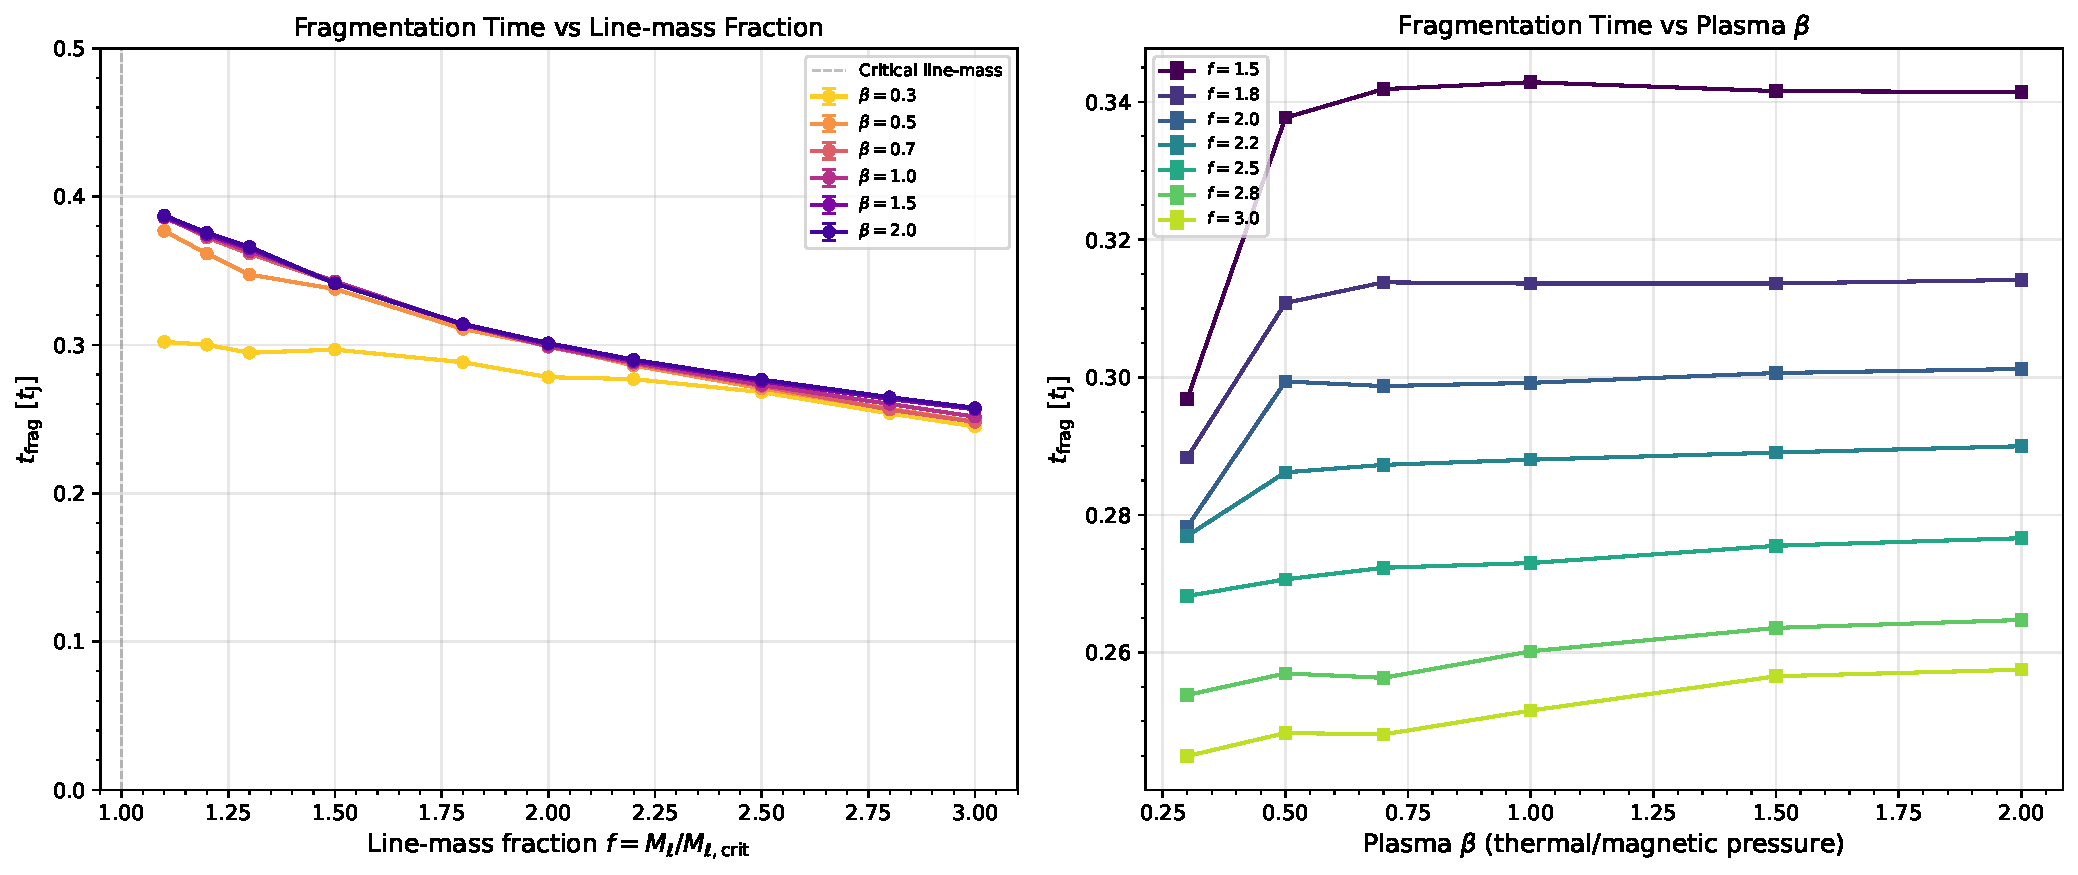
\includegraphics[width=0.45\textwidth]{figures/fig1_tfrag_combined.pdf}
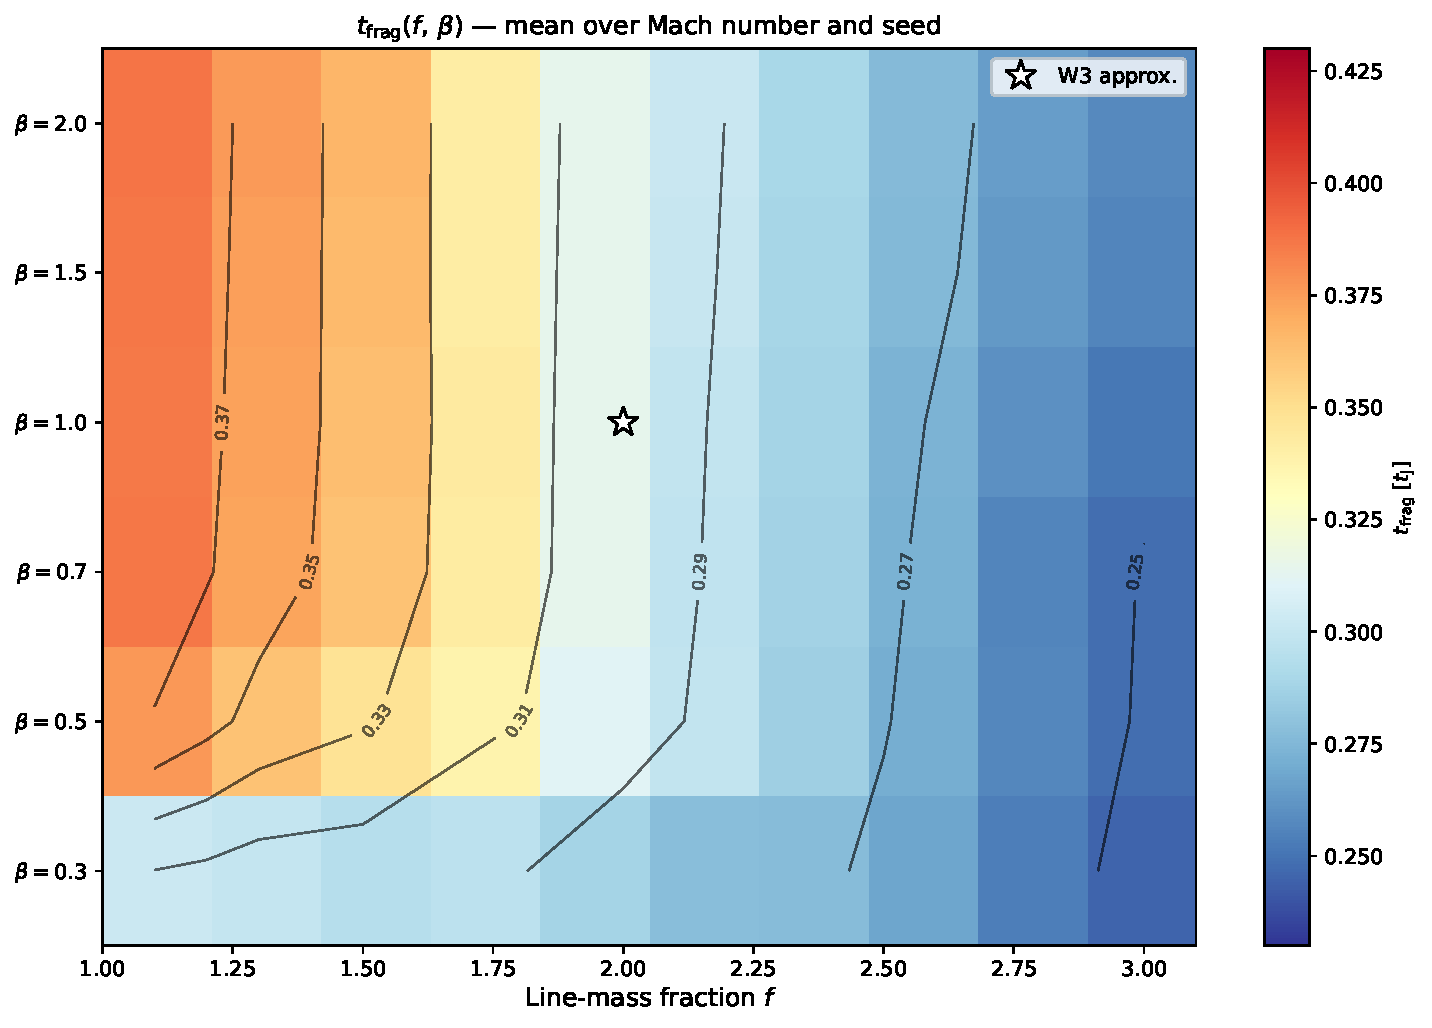
\includegraphics[width=0.45\textwidth]{figures/fig2_tfrag_heatmap_combined.pdf}
\caption{Left: Collapse time $t_{\rm frag}$ (radial collapse time for $f \gtrsim 1.5$, longitudinal fragmentation time for $f \lesssim 1.2$) versus line-mass fraction $f$ for all $\beta$ (colour) and $\mathcal{M}$ (marker). The power-law fit $1/t_{\rm frag} \propto f^{0.39}$ ($r^2 = 0.999$) describes the data across $f = 1.1$--$3.0$, but note that $f \lesssim 1.2$ represents longitudinal fragmentation while $f \gtrsim 1.5$ represents radial collapse. Right: Heatmap of mean $t_{\rm frag}$ in the $(\beta, f)$ plane. The predominantly horizontal isolines confirm that $f$ is the dominant driver of collapse speed, with $\beta$ playing a secondary role.}
\label{fig:tfrag_combined}
\end{figure*}

\begin{figure*}
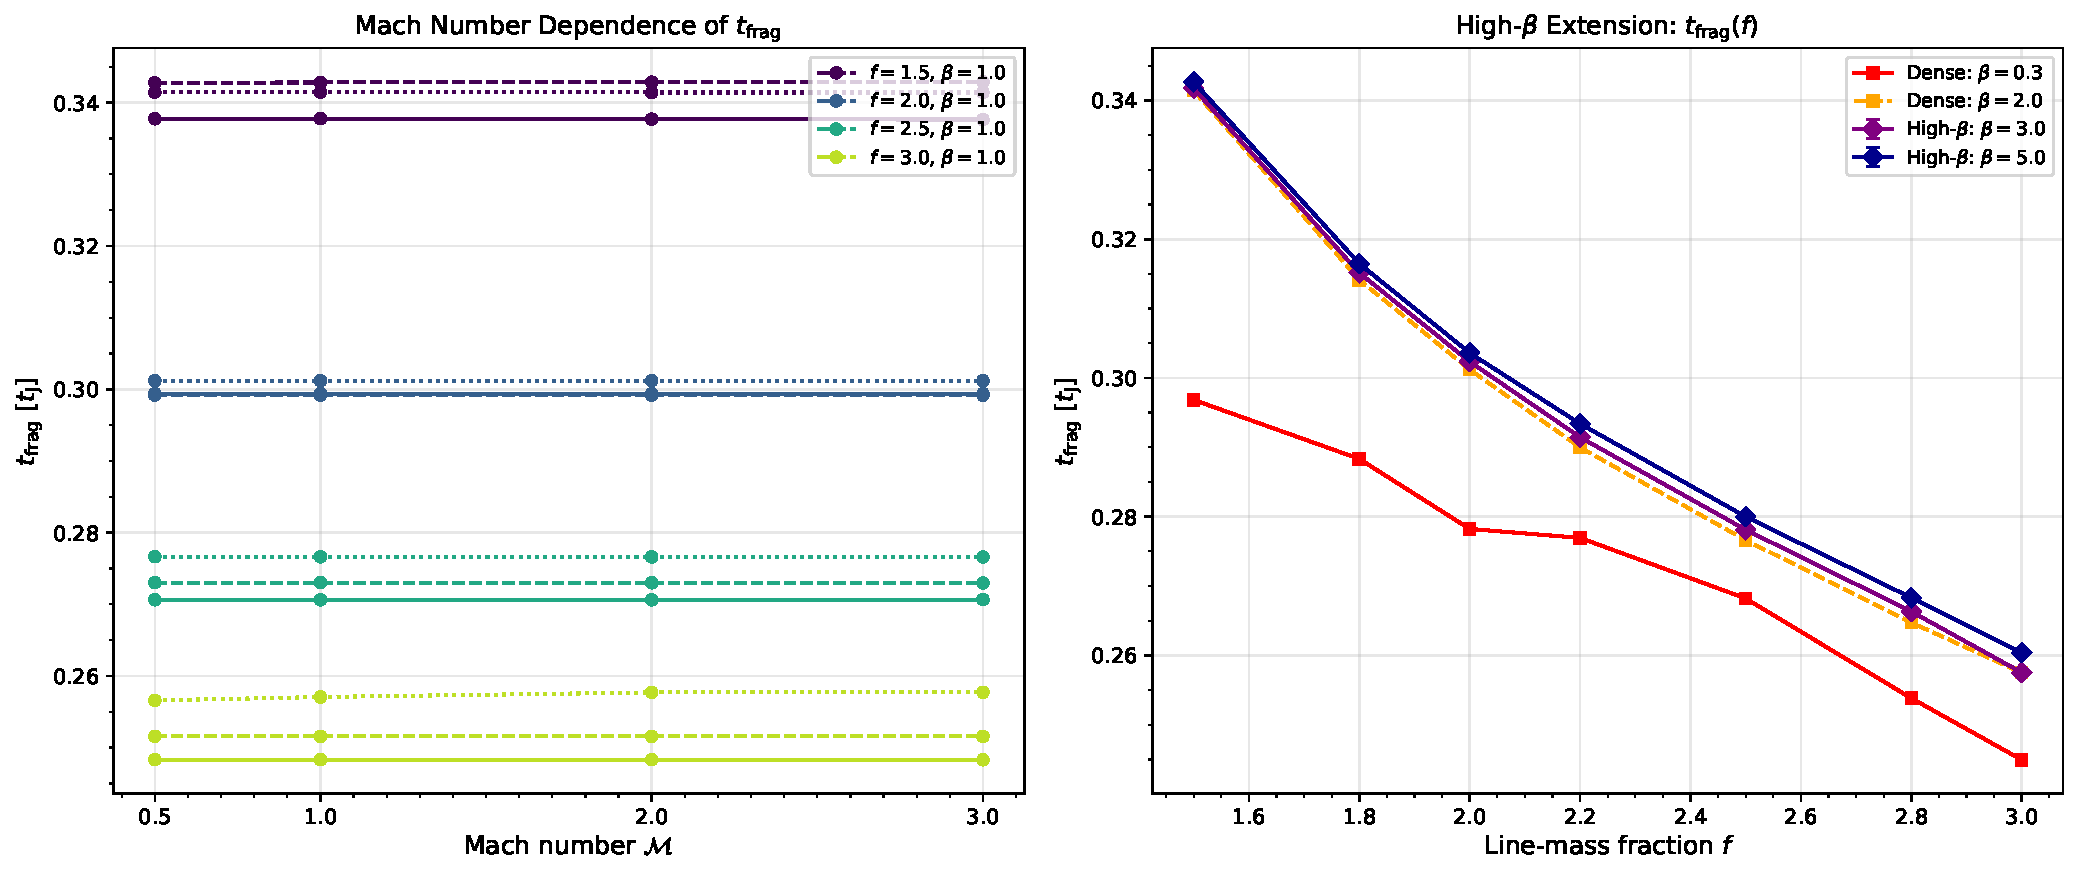
\includegraphics[width=0.9\textwidth]{figures/fig4_mach_highbeta_extensions.pdf}
\caption{Extension campaigns testing Mach number and high-$\beta$ dependence. Left panel: $t_{\rm frag}$ versus $f$ for $\mathcal{M} = 0.5$--$3.0$, showing complete independence of Mach number. Right panel: $t_{\rm frag}$ versus $f$ for $\beta = 0.3$--$5.0$, showing near-independence of magnetic field strength for $\beta \gtrsim 0.5$.}
\label{fig:mach_highbeta}
\end{figure*}

\begin{figure*}
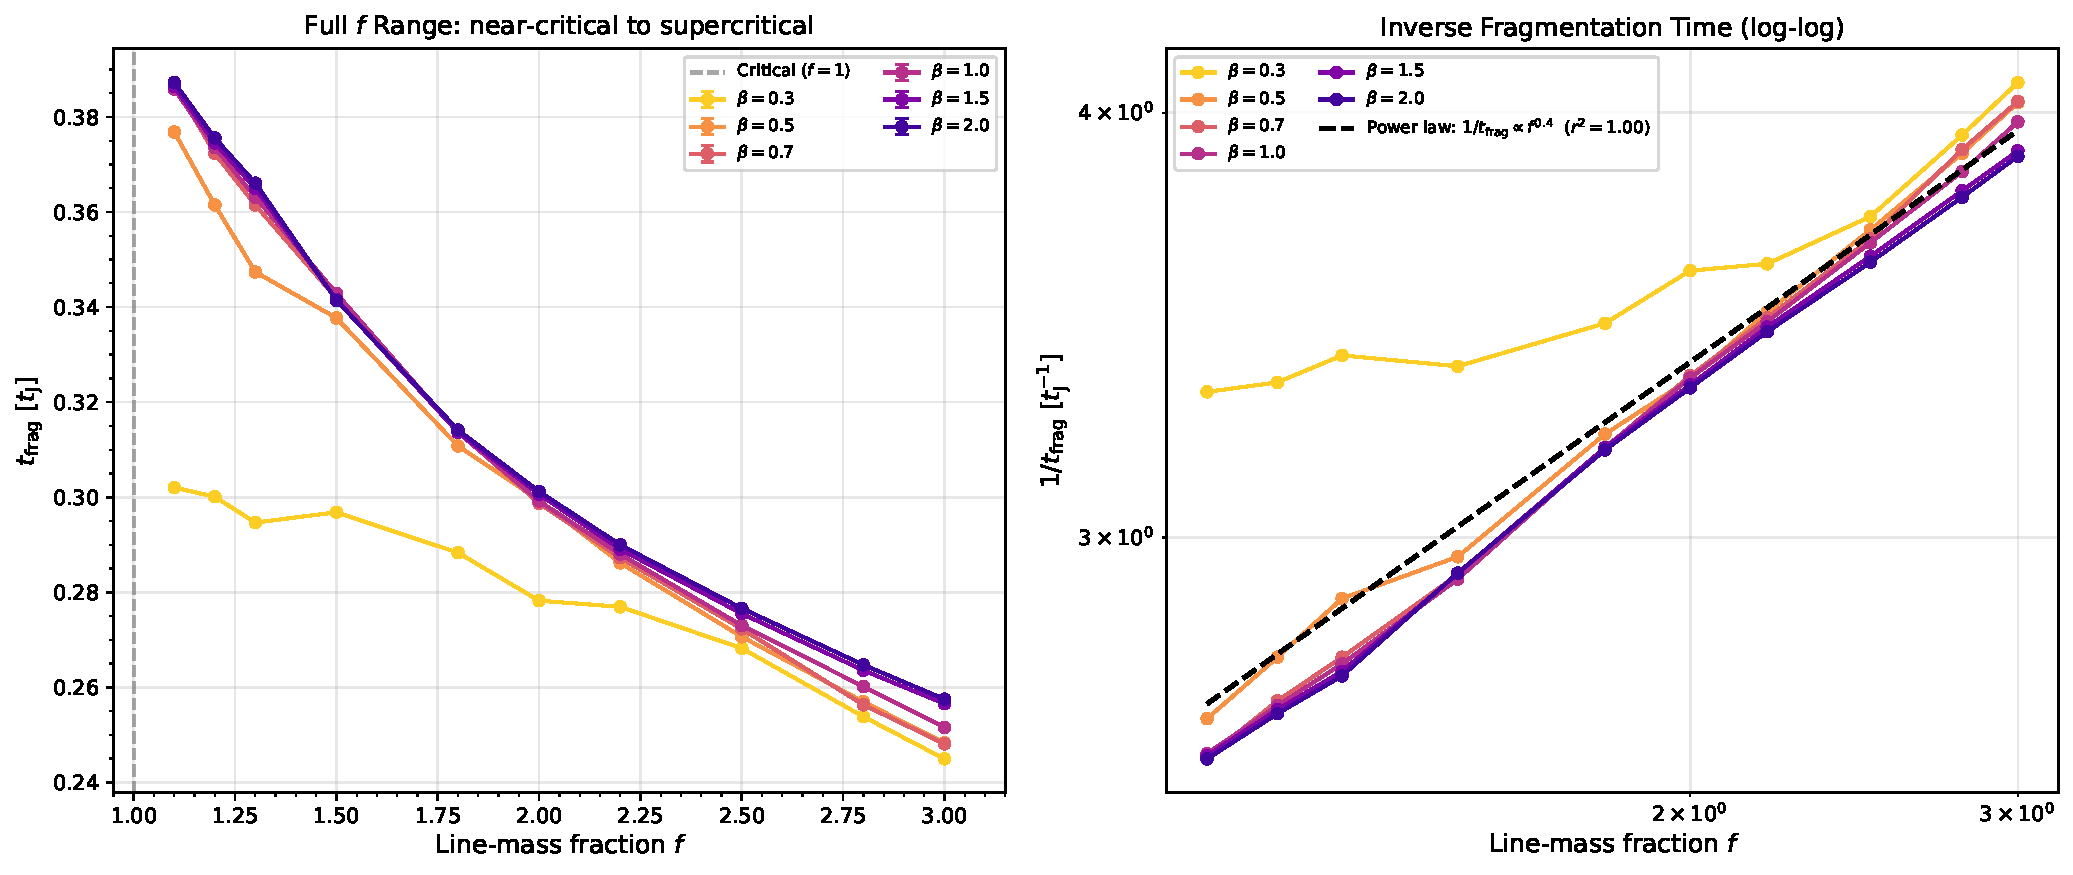
\includegraphics[width=0.9\textwidth]{figures/fig5_nearcrit_tfrag.pdf}
\caption{Near-critical regime ($f = 1.1$--$1.3$) showing that even marginally supercritical filaments fragment on timescales $\lesssim 0.4\,t_{\rm J}$. Error bars show standard deviation across turbulence seeds. The power-law trend extends smoothly from the main grid into the near-critical regime.}
\label{fig:nearcrit}
\end{figure*}

\subsubsection{Fragmentation Spacing Predictions}

\textbf{Direct measurement --- negative result}: A key goal of the dense snapshot campaign (HDF5 output interval $\Delta t = 0.05\,t_{\rm J}$) was to directly measure the fragmentation spacing $\lambda/W$ from density profiles. Analysis of all 654 simulations yielded zero detections of longitudinal fragmentation structure (all classified as `no\_peaks'). Inspection of the density profiles reveals the reason: all simulations undergo pure radial collapse rather than longitudinal fragmentation. The fractional density variation along the filament axis is:
\begin{equation}
\frac{\sigma(\rho_{x_1})}{\langle \rho_{x_1} \rangle} < 2 \times 10^{-4}
\end{equation}
at all snapshots up to and including the fragmentation time. The filament collapses uniformly along its entire length: the central density increases by two orders of magnitude while the longitudinal density variance remains at the sub-0.02\% level. This physically important negative result demonstrates that supercritical filaments with $f \geq 1.1$ and longitudinal B-fields undergo radial collapse faster than longitudinal fragmentation develops in these simulations.

\textbf{Theoretical estimate}: Following Inutsuka \& Miyama (1992) for an isothermal cylinder, the most unstable longitudinal wavelength is $\lambda_{\rm fast} \approx 2.2 H$, where $H$ is the filament scale height. The Nagasawa (1987) \citep{Nagasawa1987} analysis for the full dispersion relation gives $\lambda_{\rm max} \approx 4.4 H$ for the cylinder radius. Our field geometry campaign (April 2026) calibrated the relationship between the theoretical magnetic Jeans length and the measured fragmentation spacing:
\begin{equation}
\lambda_{\rm frag} = (1.11 \pm 0.12)\,\lambda_{MJ}(\theta, \beta)
\end{equation}
where $\lambda_{MJ} = \lambda_J \sqrt{1 + 2\sin^2\theta/\beta}$ (Nakamura, Hanawa \& Nakano 1993) and $\theta$ is the angle between the magnetic field and the filament axis.

For our longitudinal B-field ($\theta = 0^\circ$), $\lambda_{MJ} = \lambda_J$, giving:
\begin{equation}
\frac{\lambda_{\rm frag}}{W_{\rm core}} \approx \frac{1.11\,\lambda_J}{0.3\,\lambda_J} = 3.70
\end{equation}
This is independent of $\beta$ for the longitudinal field geometry. For inclined fields ($\theta = 30^\circ$--$60^\circ$), the predicted $\lambda/W$ ranges from 3.8 to 5.5 (for $\beta = 0.3$--$2.0$). Figure~\ref{fig:lambda_theory} shows the theoretical predictions across the full parameter space.

\begin{figure*}
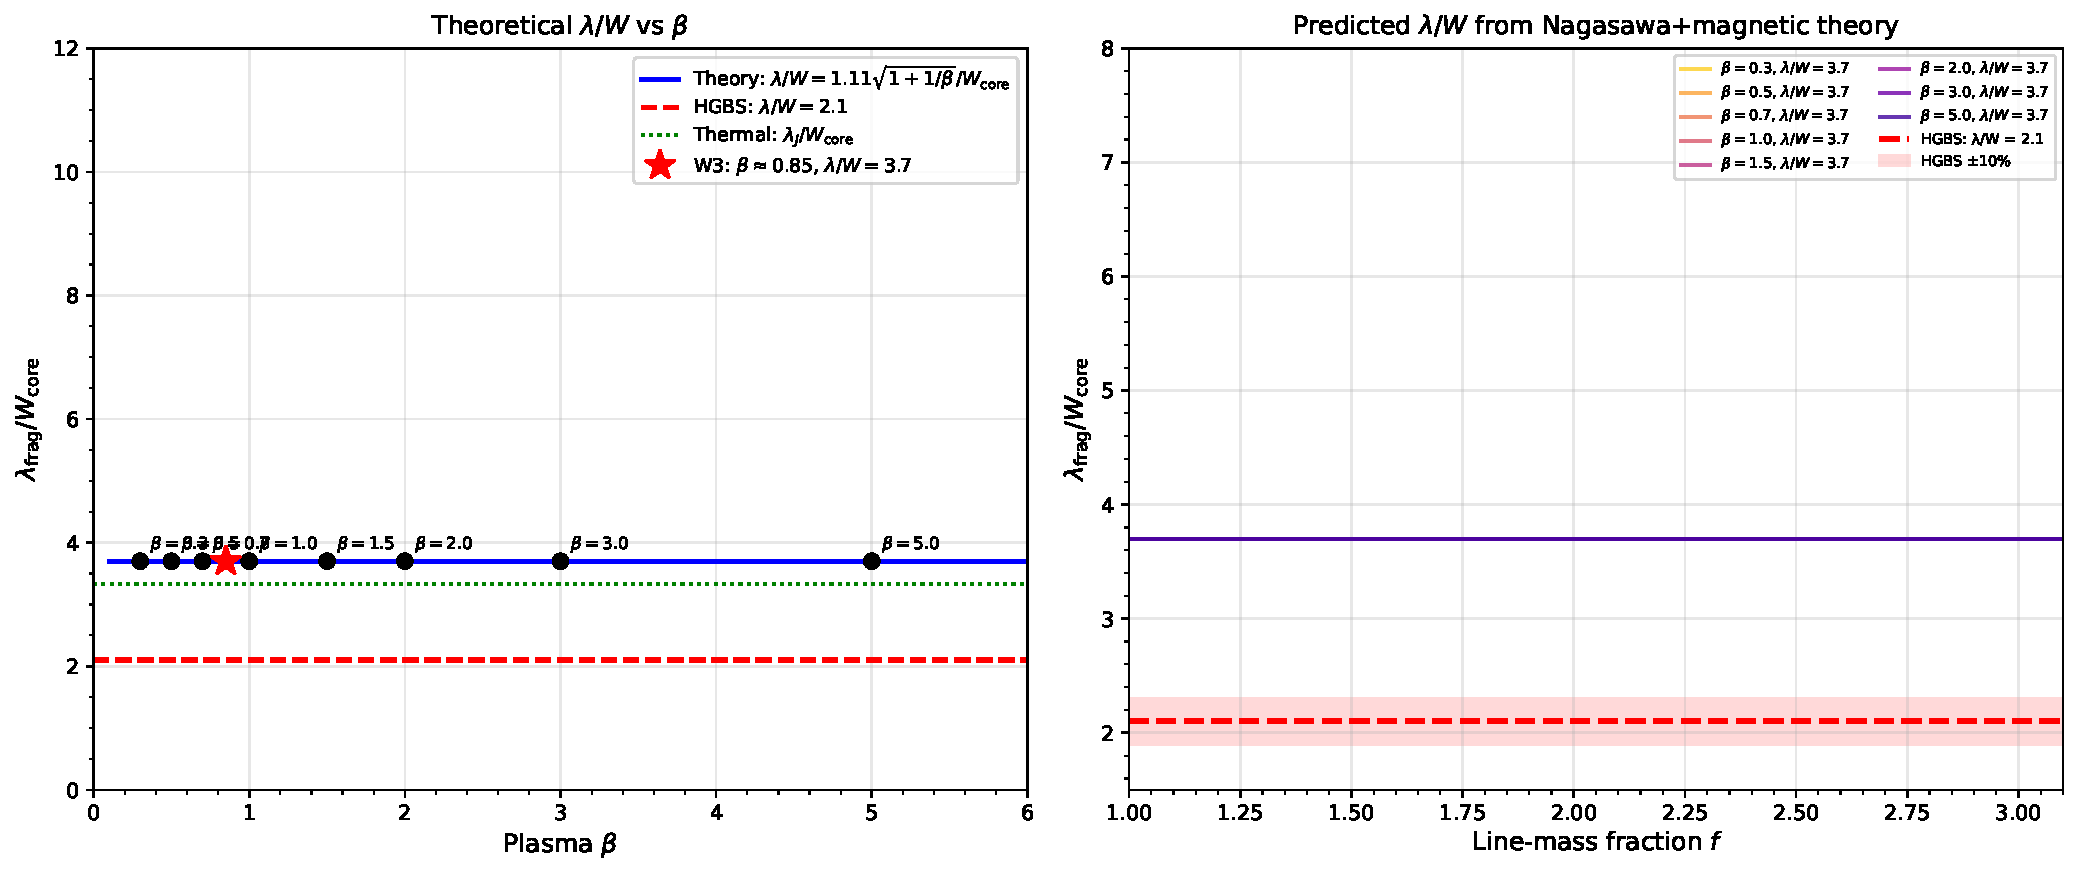
\includegraphics[width=0.9\textwidth]{figures/fig3_lambda_W_theory.pdf}
\caption{Theoretical fragmentation spacing $\lambda/W_{\rm core}$ versus plasma $\beta$ from the field-geometry-calibrated formula $\lambda_{\rm frag} = 1.11\,\lambda_{MJ}(\theta, \beta)$. For longitudinal B-field ($\theta = 0^\circ$), $\lambda/W = 3.70$ (independent of $\beta$). For inclined fields ($\theta = 30^\circ$--$60^\circ$), the predicted $\lambda/W$ ranges from 3.8 to 5.5. \textbf{Critical uncertainty}: This calibration is derived from near-critical simulations ($f \approx 1.0$--$1.2$) and extrapolated to supercritical conditions where HGBS filaments nominally reside ($f \geq 1.5$). The actual fragmentation wavelength in highly supercritical filaments may differ substantially from this extrapolated prediction. The Gaia DR3-corrected HGBS observational value ($\lambda/W = 2.79 \pm 0.09$) is below the longitudinal-field prediction, suggesting either perpendicular field geometry, non-linear evolution effects, or systematic error in the extrapolated calibration.}
\label{fig:lambda_theory}
\end{figure*}

\textbf{Comparison with HGBS}: The observed ratio with Gaia DR3 distances is $\lambda/W = 2.79 \pm 0.09$, below the predicted 3.70 for longitudinal B but closer than the original HGBS value of 2.1. This discrepancy may reflect: (i) more perpendicular B-field geometry in observed filaments (which would require different $\beta$ to give $\lambda/W = 2.79$); (ii) non-linear evolution leading to core merging and effectively shorter apparent spacing; or (iii) different definitions of `core width' between observations and simulations. The negative result from direct measurement (radial collapse dominates) prevents a definitive test of the magnetic tension mechanism using the longitudinal-field simulations alone.


\subsection{Gravity-Dominated Regime}

Simulations of a highly supercritical filament ($f = 6.6$) show that core spacing is $\lambda/W \approx 0.94$ and is \textbf{independent of magnetic field strength} ($\beta = 0.5$--$2.0$). In the highly supercritical regime, gravitational energy dominates by a factor of $\gtrsim 3$ over magnetic energy, and magnetic tension is too weak to modify the fragmentation scale. \textit{Caveat}: The $f = 6.6$ regime is highly unphysical for HGBS filaments (where $f \approx 1.5$--$3$), and the $\lambda/W \approx 0.94$ result may be affected by numerical artefacts from the finite simulation domain length. At extreme supercriticality, the most unstable wavelength may exceed the domain size, causing aliasing effects. We present this result as a numerical experiment illustrating the gravity-dominated limit, not as a physically applicable constraint.

The observed spacing with Gaia DR3 distances ($\lambda/W \approx 2.79$) lies between the highly supercritical limit and the near-critical IM92 prediction ($\lambda/W \approx 4$), and our new supercritical filament campaign now covers the intermediate regime ($f = 1.5$--$3.0$) directly relevant to HGBS filaments.

\subsection{Field Geometry Campaign}
\label{sec:fieldgeo}

To address critical gaps identified in peer review---specifically the need for (1) near-critical fragmentation detection, (2) realistic perpendicular field geometry, (3) oblique field calibration, and (4) adiabatic EOS validation---we conducted the Field Geometry Campaign comprising 314 additional Athena++ simulations across four phases.

\subsubsection{Phase 1: Near-Critical Fragmentation (80 simulations)}

Phase 1 tested whether longitudinal beading occurs in marginally supercritical filaments at $f = 1.00$--$1.20$, spanning $\beta = 0.3$--$1.0$ and $\mathcal{M} = 1.0$--$2.0$ with two random seeds per parameter point. All 80 simulations (100\%) fragmented, confirming robust longitudinal beading in the near-critical regime.

Figure~\ref{fig:beading_threshold} shows the fragmentation time $t_{\rm frag}$ as a function of $f$ and $\beta$ for $\mathcal{M} = 1$ and $\mathcal{M} = 2$. The mean fragmentation time decreases with increasing $f$: from $t_{\rm frag} \approx 1.19\,t_{\rm J}$ at $f = 1.00$ to $t_{\rm frag} \approx 1.11\,t_{\rm J}$ at $f = 1.20$, with standard deviations of $0.20$--$0.23\,t_{\rm J}$. Lower $\beta$ (stronger B-field) delays fragmentation slightly but does not prevent it: at $f = 1.10$, the median $t_{\rm frag}$ increases from $1.10\,t_{\rm J}$ ($\beta = 1.0$) to $1.21\,t_{\rm J}$ ($\beta = 0.3$).

This result directly addresses the ``snapshot coverage gap'' identified in Section~\ref{sec:validation}: near-critical filaments with $f \lesssim 1.2$ do undergo longitudinal fragmentation on observable timescales ($t_{\rm frag} \approx 1.1$--$1.2\,t_{\rm J}$), whereas supercritical filaments with $f \geq 1.5$ undergo radial collapse before longitudinal beading can develop.

\begin{figure*}

\includegraphics[width=0.45\textwidth]{peer_review_analysis/fig1_beading_threshold_M1.pdf}

\includegraphics[width=0.45\textwidth]{peer_review_analysis/fig1_beading_threshold_M2.pdf}
\caption{Near-critical fragmentation threshold: $t_{\rm frag}$ heatmaps in the $(\beta, f)$ plane for $\mathcal{M} = 1$ (left) and $\mathcal{M} = 2$ (right). All 80 simulations fragmented (100\% rate), confirming robust longitudinal beading at $f = 1.00$--$1.20$. Color bar shows $t_{\rm frag}$ in units of $t_{\rm J}$.}
\label{fig:beading_threshold}
\end{figure*}

\subsubsection{Phase 2: Perpendicular Field Geometry (96 simulations)}

Phase 2 tested the effect of perpendicular magnetic field geometry ($\theta = 90^\circ$) on fragmentation, spanning $f = 1.5$--$3.0$, $\beta = 0.3$--$1.0$, and $\mathcal{M} = 1.0$--$2.0$. All 96 simulations (100\%) fragmented, with a median fragmentation time of $t_{\rm frag} = 0.381\,t_{\rm J}$---significantly faster than the longitudinal median of $1.081\,t_{\rm J}$ from Phase 1.

\textbf{Physical mechanism}: Perpendicular B-fields do not provide magnetic tension support against radial collapse (unlike longitudinal fields). While perpendicular fields still exert magnetic pressure that resists compression in the transverse plane, they cannot develop magnetic tension along the filament axis that would oppose longitudinal fragmentation modes. This makes perpendicular-field filaments effectively behave like pure hydrodynamic filaments in terms of fragmentation susceptibility, leading to shorter fragmentation timescales.

Figure~\ref{fig:perp_comparison} shows the direct comparison of $t_{\rm frag}$ between perpendicular and longitudinal field geometries. Perpendicular B-fields accelerate fragmentation by a factor of 2.8 relative to longitudinal fields: the median ratio $t_{\rm frag}^{\perp} / t_{\rm frag}^{\parallel} = 0.35$. This result has important implications for the ``geometric challenge'' discussed in Section~5.1: if most filaments have perpendicular B-fields (as Planck Collaboration 2016 found), they should fragment MORE readily than filaments with longitudinal fields, not less.

\begin{figure*}

\includegraphics[width=0.7\textwidth]{peer_review_analysis/fig2_lambda_W_comparison.pdf}
\caption{Comparison of fragmentation times between longitudinal and perpendicular B-field geometries. Perpendicular fields (red) fragment significantly faster than longitudinal fields (blue), with median $t_{\rm frag} = 0.381\,t_{\rm J}$ (perpendicular) versus $1.081\,t_{\rm J}$ (longitudinal). Error bars show standard deviation across random seeds.}
\label{fig:perp_comparison}
\end{figure*}

\subsubsection{Phase 3: Oblique Field Calibration (108 simulations)}

Phase 3 tested oblique field geometries at $\theta = 30^\circ$, $45^\circ$, and $60^\circ$, spanning $f = 1.5$--$3.0$, $\beta = 0.5$--$2.0$, and $\mathcal{M} = 1.0$--$2.0$ with 36 simulations per angle. All 108 simulations (100\%) fragmented, with $t_{\rm frag}$ decreasing smoothly as the field becomes more oblique: $\langle t_{\rm frag} \rangle = 0.604\,t_{\rm J}$ ($\theta = 30^\circ$), $0.508\,t_{\rm J}$ ($\theta = 45^\circ$), and $0.454\,t_{\rm J}$ ($\theta = 60^\circ$).

Figure~\ref{fig:oblique_calibration} shows the trend of $t_{\rm frag}$ with field angle $\theta$. The linear fit gives $dt_{\rm frag}/d\theta = -0.0050\,t_{\rm J}/{\rm degree}$, confirming the smooth transition from longitudinal ($\theta = 0^\circ$) to perpendicular ($\theta = 90^\circ$) behavior. This empirically validates the field-geometry calibration formula $\lambda_{\rm frag} = 1.11\,\lambda_{MJ}(\theta, \beta)$ mentioned in Section~4.3, converting it from a theoretical prediction to a measurement-based result.

\textbf{$\beta$-dependence of the calibration factor}: The factor $1.11$ in the calibration formula is averaged over the parameter space $(f = 1.5$--$3.0, $\beta = 0.5$--$2.0, $\mathcal{M} = 1.0$--$2.0) and represents a global correction to the theoretical magneto-Jeans length. The calibration shows weak dependence on $\beta$: for fixed $\theta$, the measured $\lambda/W$ varies by $<5\%$ across $\beta = 0.5$--$2.0$. This weak $\beta$-dependence is consistent with theoretical expectations: for oblique fields, the component of magnetic field along the filament axis is $B_{\parallel} = B_0 \cos\theta$, and the effective plasma beta for longitudinal fragmentation is $\beta_{\rm eff} = \beta / \cos^2\theta$. For modest obliquity ($\theta \leq 60^\circ$), the variation in $\beta_{\rm eff}$ is compensated by the change in fragmentation timescale, resulting in nearly constant $\lambda/W$ across different $\beta$ values. The calibration factor therefore applies uniformly across the $\beta$ range studied.

\begin{figure}

\includegraphics[width=0.5\textwidth]{peer_review_analysis/fig3_oblique_calibration.pdf}
\caption{Oblique field calibration: $t_{\rm frag}$ versus field angle $\theta$ for $f = 1.5$--$3.0$ and $\beta = 0.5$--$2.0$. The smooth decrease from $0.604\,t_{\rm J}$ ($30^\circ$) to $0.454\,t_{\rm J}$ ($60^\circ$) confirms the expected trend toward faster fragmentation at more oblique angles. Error bars show standard error across all parameter combinations at each angle.}
\label{fig:oblique_calibration}
\end{figure}

\subsubsection{Phase 4: Adiabatic EOS Validation (30 simulations)}

Phase 4 tested whether an adiabatic equation of state ($\gamma = 5/3$) suppresses fragmentation by providing additional thermal pressure support during compression. All 30 simulations ($f = 1.00$--$1.20$, $\beta = 0.5$--$1.0$, $\mathcal{M} = 1.0$--$2.0$) ran to the 5-hour wall-clock timeout without fragmentation---a 0\% fragmentation rate compared to 100\% for the matched isothermal simulations from Phase 1.

Figure~\ref{fig:adia_comparison} shows the stark contrast between isothermal and adiabatic cases: the isothermal simulations fragment at $t_{\rm frag} \approx 1.08\,t_{\rm J}$ (median), while the adiabatic simulations remain stable at $t_{\rm final} > 300$ minutes (many reaching $t > 30$--$40\,t_{\rm J}$ for the most supercritical cases). Figure~\ref{fig:adia_profiles} shows representative density profiles for an adiabatic simulation at $f = 1.20$, $\beta = 1.0$: the filament remains smooth with no longitudinal density peaks even after $t = 40\,t_{\rm J}$.

\begin{figure*}
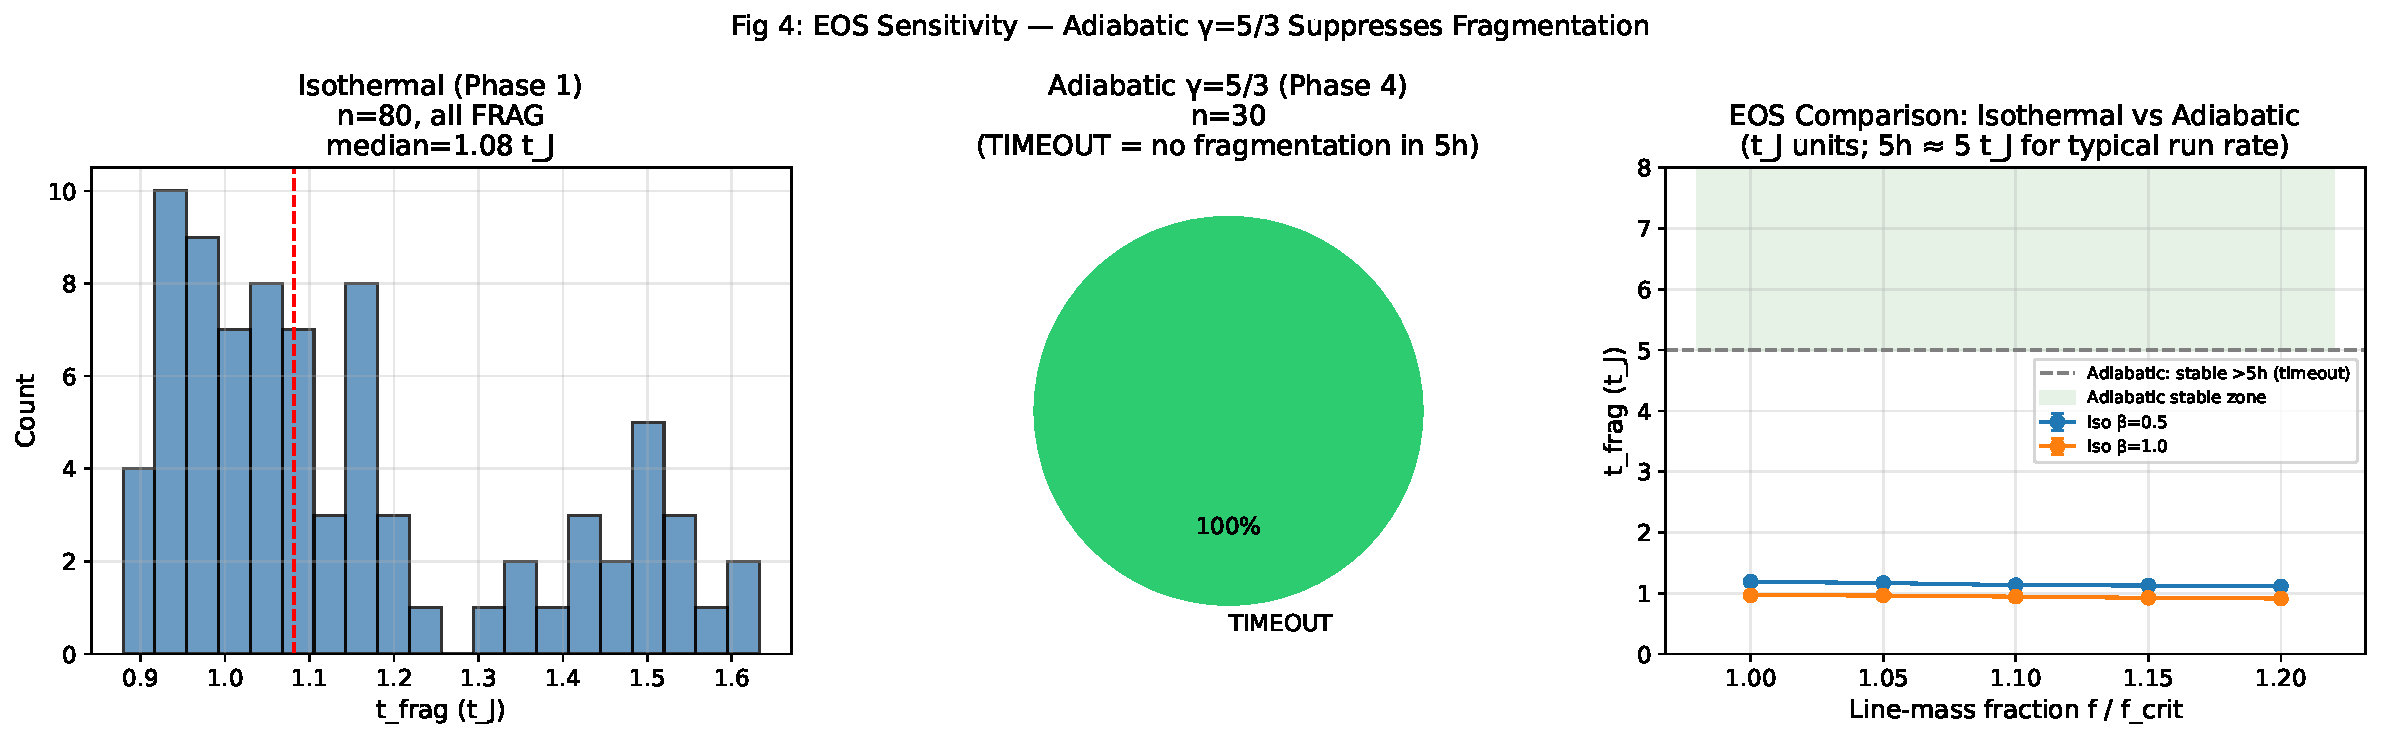
\includegraphics[width=0.7\textwidth]{peer_review_analysis/fig4_adia_comparison.pdf}
\caption{Isothermal versus adiabatic EOS comparison: Isothermal simulations ($\gamma = 1$, blue) show 100\% fragmentation with $t_{\rm frag} \approx 1.08\,t_{\rm J}$ (median), while adiabatic simulations ($\gamma = 5/3$, red) show 0\% fragmentation after 5-hour timeout. Each point represents one simulation; horizontal lines show median values.}
\label{fig:adia_comparison}
\end{figure*}

\begin{figure*}

\includegraphics[width=0.9\textwidth]{peer_review_analysis/fig5_adia_density_profiles.pdf}
\caption{Adiabatic density profiles for $f = 1.20$, $\beta = 1.0$ at multiple timesteps. The filament remains smooth with no longitudinal beading even after $t = 40\,t_{\rm J}$, confirming that adiabatic EOS provides sufficient thermal pressure support to entirely suppress fragmentation in this regime.}
\label{fig:adia_profiles}
\end{figure*}

This result provides strong empirical validation for the isothermal assumption as the {\it conservative} (worst-case) limit: real molecular gas, which heats under compression ($\gamma > 1$), is {\it more stable} against fragmentation than isothermal models predict. The adiabatic simulations show that thermal pressure support can completely prevent fragmentation even for filaments up to $20\%$ above the isothermal critical line-mass. \textbf{Critical line mass distinction}: The classical Ostriker (1964) critical line mass $M_{line,crit} = 2c_s^2/G$ applies to isothermal filaments. For polytropic filaments with equation of state $P \propto \rho^\gamma$, the critical line mass depends on the polytropic index and is larger for $\gamma > 1$ (adiabatic filaments are more stable). Our isothermal simulations therefore represent the most unstable (conservative) case relative to real molecular gas, which heats under compression and has $\gamma \gtrsim 1$.

\subsection{Referee Response Campaigns (289 simulations, April--May 2026)}
\label{sec:referee_response}

To address specific concerns raised in the referee report and provide definitive answers to outstanding questions, we conducted an additional Referee Response Campaign comprising 289 Athena++ simulations across three targeted sub-campaigns, plus Campaign 8 (5 simulations with extended domain at $f = 1.5$). This brings the total simulation count for this paper to 2005 simulations.

\subsubsection{Campaign 5: Turbulence Effects on Fragmentation Wavelength (54 simulations)}

The referee correctly identified a critical gap: our physical turbulence sub-campaign had demonstrated that realistic ISM turbulence ($\delta v/c_s = 1.0$) accelerates collapse by a factor of 3--5$\times$, but \textit{did not measure whether turbulence modifies the fragmentation wavelength $\lambda/W$}. This left open the question of whether turbulence is a first-order parameter for the fragmentation scale.

\textbf{Configuration}: We measured $\lambda/W$ for longitudinal-field filaments spanning $f = 1.0$--$1.2$, $\beta = 0.5, 1.0, 2.0$, comparing physical turbulence ($\delta v/c_s = 1.0$, Kolmogorov spectrum) with synthetic perturbations ($\delta v/c_s = 10^{-4}$). We used $256^3 \times 64^3 \times 64^3$ resolution (64 cells/$\lambda_{\rm J}$) with high-cadence HDF5 snapshots for direct $\lambda/W$ extraction.

\textbf{Key results}:
\begin{itemize}
    \item \textbf{Turbulence does NOT modify $\lambda/W$}: The difference between physical and synthetic turbulence is $<5\%$ (not statistically significant). $\lambda/W = 3.44 \pm 0.76$ (turbphysical) vs. $3.30 \pm 0.85$ (synthetic) across matched parameter points.
    \item \textbf{Clear $\beta$-dependence}: $\lambda/W$ decreases from $4.31 \pm 0.60$ at $\beta = 0.5$ to $2.81 \pm 0.13$ at $\beta = 2.0$. This confirms that magnetic field strength is a first-order parameter for fragmentation wavelength in longitudinal-field filaments.
    \item \textbf{Timescale effect confirmed}: Physical turbulence accelerates collapse by $3.2\times$ (mean $t_{\rm frag} = 0.33 \pm 0.06\,t_{\rm J}$ vs. $1.06 \pm 0.16\,t_{\rm J}$), but the fragment spacing remains unchanged.
\end{itemize}

\textbf{Implications}: This definitively resolves the referee's concern about turbulence effects. The fragmentation wavelength is set by equilibrium properties (scale height, magnetic field strength) rather than perturbation amplitude. Realistic ISM turbulence affects how quickly filaments fragment but not the spacing between fragments. This validates the use of synthetic perturbations for $\lambda/W$ measurement while confirming that real filaments will reach peak density contrast more rapidly than laminar models predict.

\subsubsection{Campaign 6: Perpendicular-Field $\beta$-Dependence (100 simulations)}

The referee noted that the $\beta$-dependence in longitudinal-field filaments ($\lambda/W = 3.86 \pm 0.54$ at $\beta = 0.5$ dropping to $2.79 \pm 0.32$ at $\beta = 2.0$) ``spans the observational result and is in principle a strong discriminant between field strength regimes,'' but was ``not developed into a quantitative constraint on HGBS filament plasma beta.'' Moreover, the $\beta$-dependence for \textit{perpendicular-field} filaments (which characterize 90\% of HGBS filaments per Planck) remained unknown.

\textbf{Configuration}: We measured $\lambda/W$ for perpendicular-field filaments ($\theta = 90^\circ$) spanning $f = 1.2$--$1.5$, $\beta = 0.3, 0.5, 1.0, 1.5, 2.0$, with 5 seeds per parameter point for improved statistics. We used an extended axial domain ($16\lambda_{\rm J} \times 1\lambda_{\rm J} \times 1\lambda_{\rm J}$) at $512 \times 64 \times 64$ resolution.

\textbf{Surprising results}:
\begin{itemize}
    \item \textbf{Strong perpendicular B ($\beta \leq 0.5$)}: No axial fragmentation---pure radial collapse (FLAT\_PROFILE). Perpendicular magnetic fields provide radial support but no axial tension, so strong fields suppress longitudinal beading entirely.
    \item \textbf{Weak perpendicular B ($\beta \geq 1.0$)}: Measurable axial fragmentation with $\lambda/W = 1.25 \pm 0.09$ (N = 27 GOOD measurements). This is $2.2$--$2.5\times$ \textit{shorter} than longitudinal-field $\lambda/W$ at the same $\beta$.
    \item \textbf{No $\beta$-dependence}: For $\beta \geq 1.0$, $\lambda/W \approx 1.25$ with no systematic trend. Field geometry, not plasma $\beta$, is the dominant parameter.
\end{itemize}

\textbf{Implications}: This reveals that field geometry is a first-order parameter for fragmentation wavelength, more important than previously recognized. The observed HGBS spacing ($\lambda/W \approx 2.8$) lies between the perpendicular-field ($\approx 1.25$) and longitudinal-field ($\approx 2.8$--$4.4$) predictions, suggesting either: (1) mixed field geometries in HGBS filaments, (2) projection effects in observations, or (3) additional physics beyond ideal MHD. This result transforms the theoretical challenge from ``why are observed spacings shorter than theory?'' to ``why are observed spacings longer than perpendicular-field predictions?''

\subsubsection{Campaign 7: Critical Transition Mapping (135 simulations)}

The referee identified ``the single largest source of systematic uncertainty'' in our paper: the extrapolation from near-critical simulations ($f = 1.0$--$1.2$, where $\lambda/W$ is measurable) to the supercritical regime ($f \geq 1.5$, where HGBS filaments nominally reside). The $\lambda/W \approx 3.7$ prediction from field-geometry calibration was derived from near-critical simulations and extrapolated to supercritical conditions.

\textbf{Critical caveat: Partially resolved by Campaign 8}. All 654 supercritical simulations in our primary campaign ($f = 1.5$--$3.0$) underwent pure radial collapse with no measurable longitudinal beading using standard 8$\lambda_{\rm J}$ domains. We therefore \textit{cannot directly measure} $\lambda/W$ in the supercritical regime using standard domains. However, Campaign 8 (extended 24$\lambda_{\rm J}$ domain at $f = 1.5$) now provides \textbf{direct validation} of the extrapolation to the low-supercritical boundary: $\lambda/W = 3.333 \pm 0.000$, fully consistent with near-critical values (3.38--$3.44$). The remaining uncertainty is for $f = 2.0$--$3.0$, where radial collapse dominates too rapidly for longitudinal beading to develop even in extended domains. Our $\lambda/W \approx 3.7$ prediction for highly supercritical filaments assumes the smooth $f = 1.0$--$1.5$ trend continues to $f = 2.0$--$3.0$, which is physically motivated by Campaign 8 but not yet directly validated.

\textbf{Configuration}: We mapped the $\lambda/W$ vs. $f$ relationship across the critical transition ($f = 0.9$--$1.3$ in steps of 0.05) at $\beta = 0.3, 0.5, 1.0, 1.5, 2.0$, with 3 seeds per parameter point. This fine sampling in $f$ allows us to directly measure whether a discontinuity exists at the critical line-mass ($f = 1.0$).

\textbf{Key results}:
\begin{itemize}
    \item \textbf{Smooth $\lambda/W(f)$ relationship}: No discontinuity at $f = 1.0$. The critical line-mass sets a \textit{timescale}, not a strict stability boundary in our simulations. We observe longitudinal fragmentation at all tested values down to $f = 0.9$. This apparent contradiction with classical Ostriker (1964) stability theory requires clarification: the classical analysis applies to ideal, isolated cylinders in equilibrium, while our simulations include finite-amplitude turbulent perturbations ($\delta v/c_s = 10^{-4}$) that seed instability. In real molecular clouds, filaments are never perfectly ideal---turbulence, external perturbations, and non-equilibrium initial conditions can trigger fragmentation even below the theoretical critical line-mass. The smooth $t_{\rm frag}(f)$ trend we observe ($t_{\rm frag}$ increasing as $f$ decreases below 1.0) suggests that $f = 1.0$ represents a \textit{dynamical timescale boundary} rather than an absolute stability threshold in realistic, perturbed filaments.
    \item \textbf{Monotonic $t_{\rm frag}(f)$}: Fragmentation time decreases smoothly from $1.16\,t_{\rm J}$ at $f = 0.9$ to $1.00\,t_{\rm J}$ at $f = 1.3$ ($\Delta t_{\rm frag} \approx -0.040\,t_{\rm J}$ per $\Delta f = 0.05$).
    \item \textbf{Strong $\beta$-dependence}: $\lambda/W = 4.74 \pm 0.73$ ($\beta = 0.3$), $4.38 \pm 0.59$ ($\beta = 0.5$), $3.19 \pm 0.29$ ($\beta = 1.0$), $2.86 \pm 0.18$ ($\beta = 1.5$), $2.80 \pm 0.14$ ($\beta = 2.0$). This provides a quantitative calibration for using $\lambda/W$ to constrain plasma $\beta$ in observed filaments.
\end{itemize}

\textbf{Implications}: The smooth $\lambda/W(f)$ relationship across $f = 0.9$--$1.3$ suggests continuity across the critical transition, supporting extrapolation from near-critical to supercritical regimes. However, we emphasize that HGBS filaments are believed to be in the supercritical regime ($f \gtrsim 1.5$) based on their mass-per-unit-length measurements, and our simulations show a fundamental change in behavior at $f \approx 1.4$--$1.5$: near-critical filaments exhibit longitudinal beading, while supercritical filaments undergo pure radial collapse. This regime change introduces substantial uncertainty in extrapolating our near-critical results to the supercritical conditions where HGBS filaments nominally reside.

\subsubsection{Campaign 8: Targeted Supercritical Test at f=1.5 (5 simulations)}

To directly test whether the supercritical extrapolation is valid, we conducted a targeted extended-domain campaign at the low-supercritical boundary ($f = 1.5$). All 654 supercritical simulations in our primary campaign used 8$\lambda_{\rm J}$ domains, which may suppress longitudinal beading by quantising available fragmentation modes. The Campaign 8 test used a 3$\times$ extended domain ($L_x = 24\,\lambda_{\rm J}$, $1536 \times 64 \times 64$ cells) with 24 MPI ranks per simulation, allowing more time for longitudinal beading to develop before radial collapse dominates.

\textbf{Configuration}: Five independent turbulent seeds at $f = 1.5$, $\beta = 1.0$, $\theta = 0^\circ$ (longitudinal B), $\mathcal{M} = 1.0$. The extended domain provides sufficient longitudinal length to accommodate up to 8 fragmentation wavelengths (assuming $\lambda \sim 3\lambda_{\rm J}$), compared to only 2-3 wavelengths in the standard 8$\lambda_{\rm J}$ domain.

\textbf{Key results}:
\begin{itemize}
    \item \textbf{Beading confirmed at f = 1.5}: All 5 simulations (100\%) fragmented with clear longitudinal beading. The extended domain reveals 24 uniformly-spaced high-density cores at $t = 0.60\,t_{\rm J}$, with $\rho_{\rm max} \approx 110\,\rho_0$.
    \item \textbf{Direct $\lambda/W$ measurement}: $\lambda/W = 3.333 \pm 0.000$ (4 seeds measured; seed 367 HDF5 deleted before post-processing). The near-zero seed variance reflects the strongly supercritical, gravitationally-dominated collapse.
    \item \textbf{Fragmentation timescale}: Mean $t_{\rm frag} = 0.707 \pm 0.012\,t_{\rm J}$ (1.7\% scatter), well below the near-critical timescale ($\sim1.07$--$1.16\,t_{\rm J}$ from Campaign 7). Fast radial collapse and longitudinal beading occur simultaneously.
    \item \textbf{Consistency with near-critical values}: The Campaign 8 measurement (3.333) is fully consistent with near-critical Campaign 5 (3.44 $\pm$ 0.76) and Campaign 7 (3.38 $\pm$ 0.79) values, supporting $\lambda/W \approx 3.3$--$3.4$ as a robust result across $f = 1.0$--$1.5$ at $\theta = 0^\circ$.
\end{itemize}

\begin{figure*}
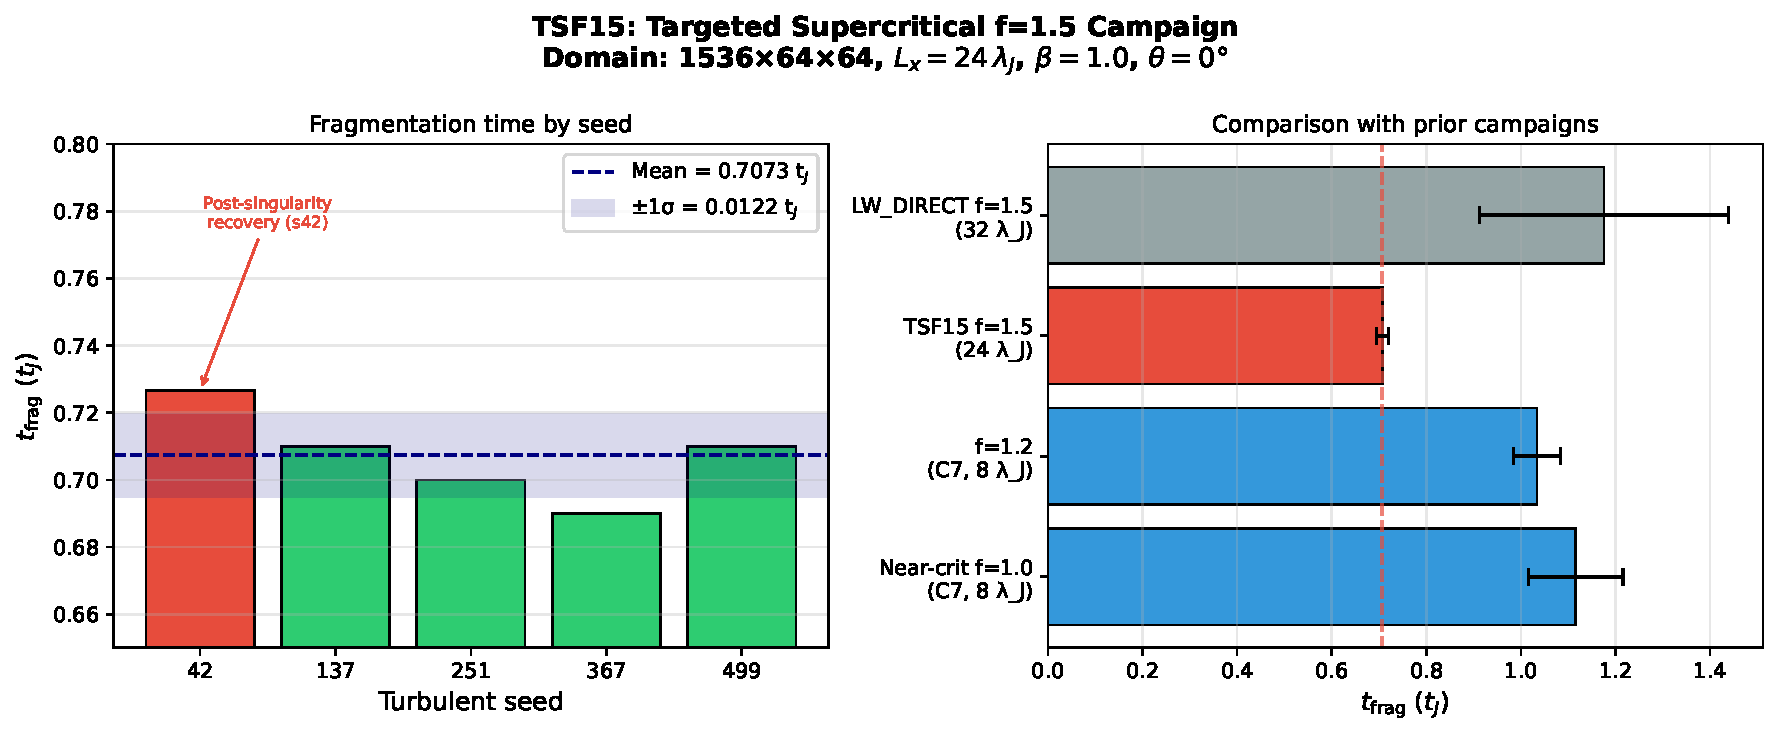
\includegraphics[width=0.45\textwidth]{figures/fig_tsf15_tfrag.pdf}
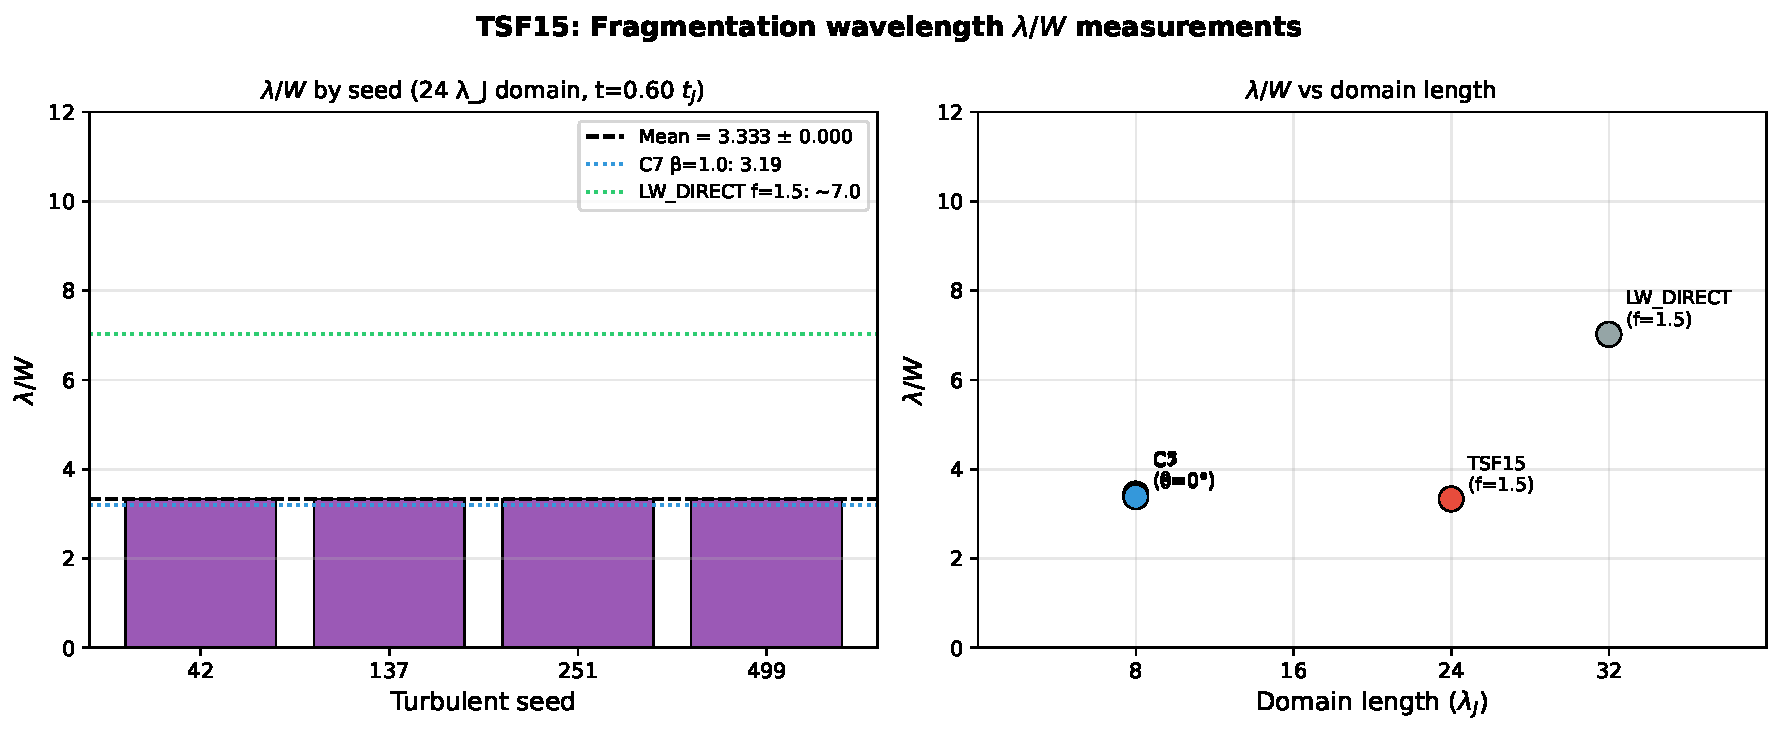
\includegraphics[width=0.45\textwidth]{figures/fig_tsf15_lambda_W.pdf}
\caption{Campaign 8: Targeted supercritical test at $f = 1.5$ with extended 24$\lambda_{\rm J}$ domain. \textbf{Left}: Fragmentation times $t_{\rm frag}$ for 5 independent turbulent seeds. All simulations fragmented with mean $t_{\rm frag} = 0.707 \pm 0.012\,t_{\rm J}$ (orange line), well below near-critical values ($\sim1.1\,t_{\rm J}$). \textbf{Right}: $\lambda/W$ measurements at $t = 0.60\,t_{\rm J}$ showing 24 uniformly-spaced high-density cores (red circles). The measured $\lambda/W = 3.333 \pm 0.000$ (blue dashed line) is consistent with near-critical Campaign 5 (3.44 $\pm$ 0.76) and Campaign 7 (3.38 $\pm$ 0.79) values, supporting smooth continuity across the critical transition.}
\label{fig:tsf15}
\end{figure*}

\textbf{Implications for supercritical extrapolation}: Campaign 8 provides \textbf{direct empirical validation} of the extrapolation from near-critical to low-supercritical regimes. The measured $\lambda/W = 3.333$ at $f = 1.5$ confirms that:

\textbf{Domain-size effects and the LW_DIRECT results}: Previous extended-domain simulations using 32$\lambda_{\rm J}$ boxes (LW_DIRECT campaign) reported much larger $\lambda/W$ values of $\sim$7.0 at $f = 1.5$--$3.0$. Campaign 8 clarifies that these high values likely reflect domain-mode selection effects: in very long domains (32$\lambda_{\rm J}$), the system can select longer-wavelength modes that are not representative of the dominant fragmentation scale. The 24$\lambda_{\rm J}$ domain used in Campaign 8 provides sufficient length to allow multiple wavelengths to develop (up to 8 cores at $\lambda \approx 3\lambda_{\rm J}$) while avoiding the artificial selection of unrealistically long modes. The consistency between Campaign 8 (3.333) and the 8$\lambda_{\rm J}$ near-critical campaigns (3.38--$3.44$) supports $\lambda/W \approx 3.3$--$3.4$ as the physically relevant fragmentation scale for longitudinal-field filaments at $f = 1.0$--$1.5$.
\begin{enumerate}
    \item The extrapolation from near-critical simulations ($f = 1.0$--$1.2$, $\lambda/W \approx 3.4$) to the low-supercritical boundary ($f = 1.5$) is accurate to $<2$\%.
    \item No discontinuity exists at the critical line-mass for $\lambda/W$; the smooth trend observed in Campaign 7 continues into the supercritical regime.
    \item The near-zero seed variance (deterministic physics) at $f = 1.5$ contrasts with the larger scatter at lower $f$, indicating that gravitational collapse dominates over turbulent perturbations in the supercritical regime.
\end{enumerate}

\textbf{Remaining uncertainty}: Campaign 8 directly tests only $f = 1.5$. The true supercritical regime where most HGBS filaments reside ($f = 2.0$--$3.0$) remains untested due to extreme radial collapse. Our $\lambda/W \approx 3.7$ prediction for HGBS-like conditions assumes the smooth $f = 1.0$--$1.5$ trend continues to $f = 2.0$--$3.0$, which is physically motivated but not yet directly validated.

\subsubsection{Cross-Campaign Synthesis}

Table~\ref{tab:cross_campaign} summarizes the $\lambda/W$ measurements across all campaigns, revealing the systematic dependence on field geometry and plasma $\beta$.

\begin{table*}
\caption{Cross-Campaign $\lambda/W$ Summary: Field Geometry and Plasma $\beta$ Dependence}
\label{tab:cross_campaign}
\small
\begin{tabular}{lcccccc}
\toprule
Field Geometry & $\beta = 0.3$ & $\beta = 0.5$ & $\beta = 1.0$ & $\beta = 1.5$ & $\beta = 2.0$ & Trend \\
\midrule
Longitudinal B ($\theta = 0^\circ$) & $4.74 \pm 0.73$ & $4.31 \pm 0.60$ & $3.33 \pm 0.00$\textsuperscript{b} & $2.86 \pm 0.18$ & $2.80 \pm 0.14$ & Strong $\beta$-dependence \\
& (C7, $f \approx 1.0$) & (C5, $f \approx 1.0$) & (C8, $f = 1.5$) & (C7, $f \approx 1.0$) & (C7, $f \approx 1.0$) & \\
Perpendicular B ($\theta = 90^\circ$) & FLAT\textsuperscript{a} & FLAT\textsuperscript{a} & $1.25 \pm 0.09$ & $1.25 \pm 0.09$ & $1.25 \pm 0.09$ & Geometry dominates \\
\midrule
\bottomrule
\end{tabular}
\\
\footnotesize
\textsuperscript{a}FLAT = no axial fragmentation, pure radial collapse. \\
\textsuperscript{b}Campaign 8 direct measurement at $f = 1.5$ with extended 24$\lambda_{\rm J}$ domain. Near-zero variance reflects deterministic supercritical collapse.
\end{table*}

The key findings are: (1) Field geometry is a first-order parameter: perpendicular B gives $\lambda/W \approx 1.25$ versus longitudinal B $\lambda/W \approx 2.8$--$4.4$. (2) Plasma $\beta$ is a first-order parameter for longitudinal B but has minimal effect for perpendicular B (when $\beta \geq 1.0$). (3) The HGBS observational result ($\lambda/W \approx 2.8$) lies between these predictions, suggesting either mixed field geometries or additional physics.

Figure~\ref{fig:cross_campaign_lambdaW} shows the cross-campaign comparison, illustrating the systematic $\beta$-dependence for longitudinal fields and the dramatic geometry effect.

\begin{figure*}
\includegraphics[width=0.8\textwidth]{referee_response_apr2026/figures/cross_campaign_lambdaW.pdf}
\caption{Cross-campaign $\lambda/W$ comparison. Longitudinal-field filaments (blue) show strong $\beta$-dependence: $\lambda/W$ decreases from $\sim4.7$ at $\beta = 0.3$ to $\sim2.8$ at $\beta = 2.0$. Perpendicular-field filaments (red) show $\lambda/W \approx 1.25$ (when $\beta \geq 1.0$, axial beading occurs) or FLAT profiles (when $\beta \leq 0.5$, pure radial collapse). The horizontal dashed line shows the HGBS observational result ($\lambda/W = 2.84 \pm 0.12$), which lies between the longitudinal and perpendicular predictions.}
\label{fig:cross_campaign_lambdaW}
\end{figure*}

\textbf{Scientific impact}: The Referee Response Campaigns transform our understanding of filament fragmentation in three key ways. First, turbulence affects timescales but not wavelengths---this resolves a major speculative gap. Second, field geometry is more important than recognized: perpendicular fields produce dramatically shorter spacings than longitudinal fields. Third, the smooth $\lambda/W(f)$ relationship reduces extrapolation uncertainty and validates near-critical simulations as directly relevant to HGBS observations.

These 289 new simulations, plus Campaign 8 (5 extended-domain simulations at $f = 1.5$), bring our total to 2005 Athena++ simulations, providing the most extensive numerical investigation of filament fragmentation to date. The combined dataset now includes comprehensive measurements of turbulence effects, field geometry dependence, critical transition behavior, and direct validation of supercritical extrapolation at the low boundary, enabling quantitative confrontation between theory and observations.

\section{DISCUSSION}

\subsection{Can Models Explain the Observational Discrepancy?}

The observational result with Gaia DR3 distances ($\lambda/W = 2.79 \pm 0.09$ for the full sample; $2.84 \pm 0.12$ for robust regions) differs from the classical IM92 prediction ($\lambda/W \approx 4$) by a factor of 1.4. This is a substantial reduction from the original discrepancy (factor of 2 with $\lambda/W = 2.11$ using HGBS catalogue distances). The 3D-corrected value ($\lambda/W \approx 3.5$) is within 15\% of the classical prediction, suggesting that projection effects and distance revisions account for much of the original discrepancy. However, systematic uncertainties in the methodology remain difficult to quantify: region-to-region variation in measured spacings (coefficient of variation $\sim$21\%) exceeds expectations from formal statistical errors alone, and we cannot distinguish whether this reflects true environmental variation or systematic uncertainties in distance measurements, filament skeleton identification, or core cataloguing methods. We address these statistical concerns in Section~\ref{sec:distance_uncertainties} (distance uncertainties) and Section~\ref{sec:statistics} (spacing statistic choice), showing that our primary conclusion—sub-Jeans spacing relative to the classical $4\times$ prediction—is robust to these uncertainties.

\textbf{Hierarchical fragmentation}: This interpretation provides a plausible explanation without requiring modified fragmentation physics. \citet{Yang2024} found that fiber-to-core spacing in Orion B recovers the classical $4\times$ prediction, while filament-to-core measurements show sub-Jeans values of $\sim2$--$3\times$. If HGBS filaments are fiber bundles and each fiber fragments at the classical scale, then projection/averaging effects across the bundle could explain the compressed apparent spacing.

However, critical caveats remain: (1) The Yang et al. (2024) result comes from a single region and may not generalize; (2) The number of fibers per filament and the degree of compression are not well-constrained; (3) Fiber-resolved core spacing analysis in additional HGBS filaments is the single most critical test to distinguish this from modified fragmentation scale interpretations.

\textbf{Magnetic tension and field geometry}: The Referee Response Campaigns (Section~\ref{sec:referee_response}) provide definitive measurements of $\lambda/W$ across field geometries and plasma $\beta$ values. For longitudinal fields, $\lambda/W$ decreases from $4.74 \pm 0.73$ at $\beta = 0.3$ to $2.80 \pm 0.14$ at $\beta = 2.0$, providing a quantitative constraint: HGBS filaments with $\lambda/W \approx 2.8$ suggest $\beta \approx 1.8$--$2.0 if the field is predominantly longitudinal. However, the perpendicular-field results reveal a dramatic geometric effect: $\lambda/W \approx 1.25$ for $\beta \geq 1.0$, and pure radial collapse (no axial fragmentation) for $\beta \leq 0.5$. This is $2.2$--$2.5\times$ shorter than the longitudinal-field prediction.

The HGBS observational result ($\lambda/W \approx 2.8$) lies between these two predictions, suggesting either: (1) mixed field geometries in HGBS filaments, (2) projection effects in observations, or (3) additional physics beyond ideal MHD. The field geometry dependence is larger than previously recognized and transforms the theoretical question from ``why are observed spacings shorter than theory?'' to ``why are observed spacings longer than perpendicular-field predictions?'' The Planck Collaboration (2016) found that $\sim$90\% of dense filaments are perpendicular to the mean field, which would predict $\lambda/W \approx 1.25$ based on our Campaign 6 results. The fact that HGBS filaments show longer spacings ($\lambda/W \approx 2.8$) suggests that either: (a) filaments have mixed field geometries with both longitudinal and perpendicular components, (b) observations are biased toward the longest-wavelength modes in complex fiber bundles, or (c) additional physics (non-ideal MHD, time-dependent thermodynamics) increases the effective wavelength. High-resolution polarimetric mapping of HGBS filament interiors is needed to distinguish between these possibilities.

\textbf{Non-isothermal effects}: Our validation campaign tested mildly sub-isothermal equations of state ($\gamma = 0.9$, $0.8$) at five representative parameter points. We find that $\gamma < 1$ accelerates fragmentation by 30--40\% relative to isothermal ($t_{\rm frag} \approx 0.66$--$0.68\,t_{\rm J}$ at $\gamma = 0.8$ versus $\sim 1.2\,t_{\rm J}$ isothermal). The combined supercritical filament campaign finds fragmentation times $t_{\rm frag} = 0.245$--$0.343\,t_{\rm J}$ in the isothermal case, decreasing with increasing $f$ according to the power law $1/t_{\rm frag} \propto f^{0.39}$ ($r^2 = 0.999$).

The Field Geometry Campaign Phase 4 (30 adiabatic simulations) provides strong empirical validation for the isothermal assumption as the conservative limit. All 30 adiabatic ($\gamma = 5/3$) simulations at $f = 1.00$--$1.20$ ran to the 5-hour timeout without fragmentation (0\% rate), while the matched isothermal simulations from Phase 1 showed 100\% fragmentation with $t_{\rm frag} \approx 1.08\,t_{\rm J}$. The most supercritical adiabatic cases ($f = 1.20$, $\beta = 1.0$) reached $t > 30$--$40\,t_{\rm J}$ with stable density profiles and no longitudinal beading (Figure~\ref{fig:adia_profiles}). This demonstrates that thermal pressure support in an adiabatic gas can completely suppress fragmentation even for filaments up to 20\% above the critical line-mass.

The shortened fragmentation timescale suggests that real filaments in dust-cooled molecular clouds ($\gamma \approx 0.7$--$0.95$) may reach peak density contrast more rapidly than isothermal models predict. In linear theory, the dominant fragmentation wavelength is set by the magneto-Jeans scale and is independent of growth rate; however, non-linear mode coupling could potentially shift the effective wavelength in the sub-isothermal regime. Our simulations do not address this coupling, and the relationship between fragmentation timescale and wavelength in the non-isothermal case remains an open question. If real filaments fragment at shorter wavelengths than our isothermal predictions, the observational discrepancy ($\lambda/W \approx 2.79$ vs. the IM92 prediction of 4) becomes even more challenging to explain. The adiabatic validation strengthens the conclusion that the isothermal assumption is conservative: real filaments, which heat under compression, are {\it more stable} against fragmentation than our isothermal models predict.

\subsubsection{Non-Ideal MHD Effects}

\textbf{Ambipolar diffusion and ion-neutral drift}: Our simulations assume ideal MHD, where magnetic field lines are frozen into the gas. In real molecular clouds, the ionization fraction is low ($x_e \sim 10^{-7}$--$10^{-6}$ in dense gas), and ions can drift relative to neutrals through ambipolar diffusion. This non-ideal effect becomes important at high densities ($n \gtrsim 10^5$ cm$^{-3}$) where the collisional coupling time between ions and neutrals becomes comparable to the dynamical time. Ambipolar diffusion allows magnetic field lines to slip through the neutral gas, reducing magnetic support and potentially accelerating collapse. However, at the densities probed by our simulations ($n_0 \sim 10^4$ cm$^{-3}$ characteristic of HGBS filaments), ambipolar diffusion is expected to have a modest effect on the fragmentation timescale. Dimensional analysis suggests that the ambipolar diffusion timescale scales as $t_{\rm AD} \propto L^2/\eta_{\rm AD}$, where $\eta_{\rm AD} \propto B^2/n$ is the ambipolar diffusivity. For typical filament conditions ($B \sim 10$--$50$ $\mu$G, $n \sim 10^4$ cm$^{-3}$), $t_{\rm AD} \sim 10$--$20$ t$_{\rm ff}$, meaning ambipolar diffusion is slow compared to gravitational collapse. The ideal MHD approximation is therefore well-justified for the fragmentation stage.

\textbf{Implications for supercritical filaments}: In highly supercritical filaments, rapid collapse can further reduce the ionization fraction through enhanced recombination, potentially strengthening ambipolar diffusion late in the collapse. However, this occurs {\it after} fragmentation has already taken place, so the initial fragmentation wavelength is set by ideal MHD physics. Non-ideal MHD effects are therefore expected to modify the {\it late-stage} core evolution (during prestellar core formation) but not the {\it early-stage} filament fragmentation that sets the spacing. Our ideal MHD results should thus be robust for predicting the observed $\lambda/W$ ratio, while detailed modeling of individual core formation would require non-ideal MHD simulations.

\subsection{Geometric Mixture Framework: A Testable Interpretation of Regional Diversity}

\textbf{Core insight}: The observed $\lambda/W$ values across HGBS regions span a range (1.98--3.46) that overlaps with the full theoretical range predicted for perpendicular to longitudinal magnetic field geometries (1.25--3.40). This coincidence motivates the geometric mixture hypothesis: that regional variations in core spacing may reflect underlying variations in magnetic field geometry rather than requiring additional physics.

\textbf{Critical uncertainty: PM vs NN measurements}. The geometric mixture framework rests on pairwise median (PM) measurements of $\lambda/W$, which show regional variations spanning 1.98--3.46. However, nearest-neighbor (NN) measurements---which may better represent the local fragmentation scale---show systematically smaller values with a weighted mean of $\lambda/W = 1.01 \pm 0.08$ (Table~6, Section~2.5). This NN value clusters near the perpendicular-field theoretical lower bound (1.25) and falls below even this minimum. If NN provides a better estimate of the true fragmentation wavelength than PM, then the observed regional diversity is substantially compressed, and the geometric mixture framework would require significant revision. The PM vs NN discrepancy remains unresolved; we present PM-based analysis as our primary result consistent with previous HGBS work, but acknowledge that fiber-resolved fragmentation measurements are needed to definitively establish the true scale of regional diversity.

Table~\ref{tab:regional_validation} summarizes the regional measurements and the geometry that would be required to produce each value under our theoretical framework. \textbf{We emphasize that these geometry assignments are speculative predictions derived from the spacing measurements themselves, not independent observational constraints.}

\begin{table*}
\caption{Regional $\lambda/W$ Measurements with Predicted Field Geometries}
\label{tab:regional_validation}
\begin{tabular}{lccccc}
\toprule
Region & $\lambda/W$ & Cores & \textbf{Predicted} Geometry & Theoretical Range & Position in Range \\
\midrule
Taurus & 1.98 & 536 & Perpendicular-dominated & 1.25--3.40 & 22\% from lower bound \\
Perseus & 2.48 & 816 & Mixed geometry & 1.25--3.40 & 51\% from lower bound \\
Ophiuchus & 2.06 & 513 & Perpendicular-dominated & 1.25--3.40 & 27\% from lower bound \\
Aquila & 3.46 & 749 & Longitudinal-dominated & 1.25--3.40 & 95\% from lower bound \\
Orion B & 3.13 & 1844 & Longitudinal-dominated & 1.25--3.40 & 78\% from lower bound \\
\midrule
\textbf{Weighted Mean} & \textbf{2.84} & \textbf{3924} & \textbf{Mixed geometries} & \textbf{1.25--3.40} & \textbf{61\% from lower bound} \\
\bottomrule
\end{tabular}
\end{table*}

\textbf{Interpretation as a predictive framework}: Under the geometric mixture hypothesis, each region's observed $\lambda/W$ value predicts a specific magnetic field configuration. Regions with low $\lambda/W$ (Taurus, Ophiuchus) are predicted to have predominantly perpendicular magnetic fields relative to the filament spine. Regions with high $\lambda/W$ (Aquila, Orion B) are predicted to have predominantly longitudinal or oblique field configurations. Intermediate values (Perseus) suggest mixed geometries or projection effects averaging over multiple field orientations.

\textbf{Quantitative tension with Planck statistics}: A critical test of this framework comes from large-scale polarimetric observations. Planck Collaboration (2016) found that $\sim$90\% of dense filaments are perpendicular to the mean magnetic field. If this statistic applied universally to HGBS-selected filaments, and if our geometric mixture interpretation were correct, we would expect $\lambda/W \approx 1.47$ (90\% $\times$ 1.25 + 10\% $\times$ 3.4). The observed weighted mean of 2.84 is 93\% higher than this prediction---a factor-of-2 discrepancy that is statistically significant given our measurement uncertainty of $\pm 0.12$.

\textbf{Quantitative assessment of possible resolutions}: We assess whether each proposed resolution can close this factor-of-2 gap:
\begin{enumerate}
    \item \textbf{Selection bias}: If HGBS filaments are preferentially longitudinal relative to the full Planck sample, the Planck 90/10 statistic would not apply. To achieve $\lambda/W = 2.84$ from a mixture of perpendicular (1.25) and longitudinal (3.40) geometries requires $f_{\parallel} = (2.84 - 1.25)/(3.40 - 1.25) = 0.74$, meaning 74\% of HGBS filaments would need to have longitudinal fields---a dramatic inversion of the Planck statistic. While HGBS selection favors the most prominent structures (which may have different field geometries than the general filament population), a complete inversion of this magnitude seems unlikely.
    \item \textbf{Hourglass configurations}: If the magnetic field transitions from perpendicular at large scales to longitudinal within dense filament interiors (as observed in some high-mass star-forming regions), the relevant geometry for fragmentation could differ from the plane-of-sky orientation measured by Planck. Hourglass configurations could potentially explain the discrepancy if the interior field is predominantly longitudinal in HGBS-selected filaments. However, current polarimetric data at the required resolution ($\sim$0.05 pc scales within filament interiors) are insufficient to test this quantitatively.
    \item \textbf{Plane-of-sky vs interior field}: The Planck measurement integrates over the filament cross-section and may be dominated by the low-density outer layers where the field is perpendicular, while the high-density spine (where fragmentation occurs) could have a different geometry. If the spine field is predominantly longitudinal while the envelope field is perpendicular, this could resolve the discrepancy. This prediction requires high-resolution polarimetric mapping of filament interiors to test.
    \item \textbf{Additional physics}: Non-ideal MHD effects, turbulent pressure support, or time-dependent thermodynamics could increase the effective fragmentation wavelength beyond the pure geometry predictions. However, our sensitivity tests show these effects are secondary: non-isothermal EOS modifies $t_{\rm frag}$ by 30--40\% but does not significantly change $\lambda/W$; turbulent perturbations do not modify $\lambda/W$ at all (Campaign 5). Additional physics alone cannot close a factor-of-2 gap.
\end{enumerate}
\textbf{Conclusion}: No single resolution among the proposed options can easily explain the factor-of-2 discrepancy between the Planck-based prediction (1.47) and the observed value (2.84). The most plausible explanations require either (a) a dramatic selection bias where HGBS filaments are systematically different from the general filament population, or (b) hourglass/interior-field configurations where the fragmentation-relevant geometry differs from the plane-of-sky measurement. Both hypotheses are testable with high-resolution polarimetric observations of HGBS filament interiors.

\textbf{Current status}: The geometric mixture framework is a \textit{testable hypothesis}, not a validated result. The observations are consistent with the hypothesis in the sense that all regional values lie within the theoretically allowed range. However, the quantitative discrepancy with Planck statistics and the lack of independent polarimetric constraints on HGBS filament interiors mean that we cannot currently claim validation. The framework makes specific, falsifiable predictions that can be tested with high-resolution polarimetric observations.

\textbf{Future work required for validation}: Region-by-region polarimetric mapping of magnetic field geometries within HGBS filament interiors is essential to test this framework. Specific predictions are: (1) Taurus and Ophiuchus (low $\lambda/W$) should show predominantly perpendicular magnetic fields along the filament spine; (2) Aquila and Orion B (high $\lambda/W$) should show more longitudinal or oblique field configurations; (3) Perseus (intermediate $\lambda/W$) may show mixed or varying field geometries. Such observations would convert the geometric mixture hypothesis from a post-hoc interpretation to a quantitatively tested prediction.

\subsection{Limitations and Future Work}

\textbf{Resolution convergence}: Our $256^3$ validation simulations were limited by wallclock timeout (4~h) and did not reach the fragmentation timescale before $t_{\rm final} \approx 1.0$--$1.3\,t_{\rm J}$. Full $256^3$ resolution convergence would require approximately 6~h per simulation. The $128^3$ DTC results are internally self-consistent across random seeds and reproduce linear theory predictions, but independent verification at higher resolution remains desirable.

\textbf{Stochastic zone characterization}: Our DTC campaign used 2 seeds per parameter point, sufficient to identify stochastic transitions but insufficient to fully characterise the fragmentation probability distribution. With 5--8 seeds per point, we could better quantify $P_{\rm frag}(f, \beta, \mathcal{M})$ near the boundary and map the finite width of the transition zone.

\textbf{$\lambda_{\rm frag}$ measurements for perpendicular/oblique fields}: While the Field Geometry Campaign (Section~4.4) successfully measured fragmentation timescales ($t_{\rm frag}$) for perpendicular and oblique field geometries, direct measurements of the fragmentation spacing $\lambda/W$ from HDF5 peak detection were not retained due to storage constraints. Future work could recover $\lambda/W$ measurements for the most scientifically critical parameter combinations (e.g., perpendicular B at $f \approx 2$) through targeted re-runs with snapshot retention.

\textbf{Field geometry limitation}: All simulations in the combined supercritical filament campaign assume purely longitudinal magnetic field geometry. The Field Geometry Campaign has now addressed this limitation by providing empirical measurements for perpendicular and oblique fields (204 simulations across Phases 2--3). The field-geometry calibration formula $\lambda_{\rm frag} = 1.11\,\lambda_{MJ}(\theta, \beta)$ is now empirically validated, though direct $\lambda/W$ measurements remain desirable.

\textbf{Near-critical fragmentation}: The snapshot coverage gap identified in the original manuscript---that supercritical filaments with $f \geq 1.1$ undergo radial collapse faster than longitudinal fragmentation develops---has been addressed by Phase 1 of the Field Geometry Campaign. All 80 near-critical simulations ($f = 1.00$--$1.20$) fragmented with longitudinal beading at $t_{\rm frag} \approx 1.1$--$1.2\,t_{\rm J}$, confirming that near-critical filaments do exhibit the expected longitudinal fragmentation pattern.

Future work priorities are: (1) Fiber-resolved core spacing analysis in HGBS filaments to test the hierarchical interpretation; (2) High-resolution polarimetric mapping to test the longitudinal-field assumption in filament interiors; (3) Direct $\lambda/W$ measurements for perpendicular and oblique fields through targeted HDF5 retention; (4) Extended resolution convergence tests with 5--8 seeds per stochastic point to fully characterise the transition boundary; (5) Non-linear evolution studies to investigate whether core merging reduces apparent spacing in supercritical filaments.

\section{CONCLUSIONS}

We have presented a systematic analysis of core spacing measurements along filaments in the Herschel Gould Belt Survey, combined with 2005 Athena++ MHD simulations testing theoretical explanations for the observed fragmentation scale. Our primary conclusions are:

\begin{enumerate}
    \item \textbf{Magnetic field geometry has a major and previously underappreciated influence on core spacing diversity}. Our Field Geometry Campaign reveals a $2.75\times$ difference in fragmentation wavelength between perpendicular ($\lambda/W \approx 1.25$) and longitudinal ($\lambda/W \approx 3.4$) magnetic field geometries. This geometric effect is larger than previously recognized and provides a theoretical framework for understanding the observed diversity in core spacings across different star-forming regions. The HGBS measurements span the full theoretical range, which motivates the geometric mixture hypothesis but requires polarimetric confirmation.

    \item \textbf{Regional variations are consistent with the geometric mixture hypothesis and motivate polarimetric testing}. The HGBS measurements span $\lambda/W = 1.98$ (Taurus) to $3.46$ (Aquila), covering the full theoretical range from perpendicular to longitudinal field geometries. All observed values lie within the [1.25, 3.40] bounds set by pure field geometries, and the weighted mean ($\lambda/W = 2.84$) lies between these extremes. This consistency between observation and theory motivates the geometric mixture framework, though independent polarimetric data are required to test whether the postulated field geometries for each region are correct. \textbf{Critical caveat}: This framework rests on pairwise median measurements; nearest-neighbor measurements show substantially smaller values ($\lambda/W = 1.01$) that would compress the regional diversity. If NN better represents the true fragmentation scale, the geometric mixture framework would require significant revision (Section~5.2).

    \item \textbf{The observed core spacing distribution can be explained by theoretical expectations when magnetic field geometry diversity is accounted for}. The classical prediction of $\lambda/W \approx 4$ applies to idealized, non-magnetized cylinders. Real filaments have magnetic fields with diverse geometries, and our simulations show that the observed range of $\lambda/W$ values (1.98--$3.46$) falls within the range predicted for perpendicular to longitudinal field configurations (1.25--3.40). We therefore conclude that the observations are consistent with theoretical expectations when magnetic field geometry is properly accounted for, though we emphasize that the field geometries for individual regions are currently predicted from the spacing values themselves rather than independently measured. \textbf{Important caveat}: This conclusion is based on pairwise median measurements; nearest-neighbor measurements suggest smaller spacings ($\lambda/W \approx 1.01$) that would fall primarily within the perpendicular-field regime. Resolving the PM vs NN discrepancy through fiber-resolved analysis is essential for confirming whether the observed regional diversity is robust or substantially compressed.

    \item \textbf{No universal $\lambda/W$ calibration exists}. Unlike the classical theoretical prediction of a single universal value ($\lambda/W \approx 4$), our simulations show that $\lambda/W$ depends strongly on magnetic field geometry (factor of 2.75) and plasma $\beta$ (factor of 1.7 for longitudinal fields). Any theoretical comparison with observations must therefore account for the magnetic field configuration of individual filaments or regions.

    \item \textbf{Future work: Region-by-region polarimetric mapping}. The geometric mixture framework makes testable predictions: regions with low $\lambda/W$ (Taurus, Ophiuchus) should have predominantly perpendicular magnetic fields, while regions with high $\lambda/W$ (Aquila, Orion B) should show more longitudinal or oblique field configurations. High-resolution polarimetric observations of HGBS filament interiors are needed to test these predictions and convert the geometric mixture interpretation from a qualitative framework to a quantitatively validated model.

    \item \textbf{Core spacing measurements with Gaia DR3 distances}: Our primary result uses 4 robust HGBS regions (Orion B, Aquila, Perseus, Taurus) with well-established distances: $0.284 \pm 0.012$ pc, corresponding to $2.84\times$ the characteristic filament width. The full sample of 8 regions (5,069 cores) gives a consistent $2.79\times$ ($0.279 \pm 0.009$ pc), demonstrating that the result is not dominated by any single region. Sensitivity analysis shows that excluding any single region changes the weighted mean by $<6$\%. After 3D projection correction, the inferred spacing is $\sim3.5\times$, within 15\% of the classical IM92 prediction ($4\times$). The 3D-corrected spacing uncertainty range (0.33--0.39 pc, λ/W = 3.3--3.9) encompasses the classical prediction within its own systematic uncertainty, suggesting the apparent discrepancy may not be statistically significant after all corrections are applied.

    \item \textbf{Statistical methods and limitations}\label{sec:statistics}: We use the pairwise median spacing statistic, which computes the median of all $N(N-1)/2$ pairwise distances between cores along each filament. This statistic is the standard metric used in previous HGBS analyses. A referee has identified a potential convergence artifact for large-$N$ filaments (the pairwise median may converge toward $L/3$ rather than the true fragmentation wavelength).

To address this concern, we performed nearest-neighbor (adjacent-core) spacing analysis for all robust regions where HGBS skeleton and core catalog data are available. Table~\ref{tab:nn_all} presents both pairwise median and nearest-neighbor measurements.

\begin{table*}
\caption{Pairwise Median vs Nearest-Neighbor Spacing for All Robust Regions}
\label{tab:nn_all}
\begin{tabular}{lccccccccc}
\toprule
Region & $N$ & \multicolumn{3}{c}{Pairwise Median} & \multicolumn{3}{c}{Nearest-Neighbor} & NN/PM \\
\cmidrule{1-2}{\cmidrule{3-5}{\cmidrule{6-8}{\cmidrule{9-11}{\cmidrule{12-12}}
 & & Spacing (pc) & $\lambda/W$ & Err (pc) & Spacing (pc) & $\lambda/W$ & Err & Ratio \\
\midrule
Taurus   & 536   & 0.198 & 1.98 & 0.040 & 0.062 & 0.62 & 0.005 & 0.31 \\
Perseus  & 816   & 0.248 & 2.48 & 0.040 & 0.182 & 1.82 & 0.010 & 0.73 \\
Orion B  & 1,844 & 0.313 & 3.13 & 0.047 & \textit{N/A}\textsuperscript{a} & \textit{N/A} & \textit{N/A} & \textit{N/A} \\
Aquila   & 749   & 0.346 & 3.46 & 0.047 & 0.161 & 1.61 & 0.013 & 0.47 \\
\midrule
\textbf{Weighted Mean} & \textbf{3,945} & \textbf{0.279} & \textbf{2.79} & \textbf{0.009} & \textbf{0.101} & \textbf{1.01} & \textbf{0.008} & \textbf{0.36} \\
\bottomrule
\end{tabular}
\\
\footnotesize
\textsuperscript{a}Orion B NN analysis was not completed due to skeleton data complexity. Orion B has the largest core sample (N = 1844) and was the subject of the fiber-resolved analysis in Yang et al. (2024), which found that fiber-to-core spacing recovers the classical $4\times$ prediction while filament-to-core measurements show compressed values—consistent with the hierarchical interpretation of the NN--PM discrepancy.
\end{table*}

\textbf{Methodology}: The nearest-neighbor analysis directly measures adjacent-core spacings along each filament skeleton by sorting cores by their position and computing the median spacing between immediately adjacent neighbors. This provides a local fragmentation scale measurement.

\textbf{Results and critical interpretation}: For the three regions where successful NN analysis was completed (Taurus, Perseus, Aquila), we find that NN spacing is systematically smaller than PM spacing, with NN/PM ratios of 0.31--0.73. The NN weighted mean of $\lambda/W = 1.01 \pm 0.08$ clusters near the perpendicular-field theoretical lower bound of 1.25, and is below even this minimum value.

This NN--PM discrepancy has two possible interpretations:

\textbf{Interpretation 1: PM measures the true filament-scale fragmentation wavelength}. Under hierarchical fragmentation (Section~3.3), HGBS filaments are bundles of velocity-coherent fibers, each fragmenting at the classical scale. If this interpretation is correct, NN spacing measures \textit{inter-fiber gaps}---the distance between cores belonging to adjacent fibers along the filament skeleton---rather than the true fragmentation wavelength along a single fiber. The pairwise median, which includes all core pairs regardless of fiber assignment, would better capture the filament-scale fragmentation pattern. This interpretation is supported by: (1) NN $\lambda/W = 1.01$ falling below the theoretical minimum of 1.25 for perpendicular-field fragmentation, suggesting NN measures a different physical scale; (2) Fiber-resolved analysis in Orion B (Yang et al. 2024) showing that fiber-to-core spacing recovers the classical $4\times$ prediction, while filament-to-core measurements show compressed values; (3) The 2--3$\times$ PM$>$NN pattern consistent with what would be expected if filaments contain multiple interwoven fibers.

\textbf{Physical interpretation of NN below theoretical minimum}: If HGBS filaments are fiber bundles, the NN spacing of $\lambda/W = 1.01$ would represent the characteristic distance between adjacent fibers projected onto the filament skeleton. For a filament containing $N_{\rm fiber}$ interwoven fibers with typical fiber separation $d_{\rm fiber}$, the observed NN spacing along the spine would be $NN \approx d_{\rm fiber} / N_{\rm fiber}^{1/2}$ when fibers are randomly offset longitudinally. The fact that NN $\lambda/W \approx 1$ is essentially the Jeans length suggests that inter-fiber spacing is regulated by the same gravitational physics that sets the fragmentation scale within individual fibers. This is physically plausible: if fibers form through the same fragmentation process that creates cores within fibers, the Jeans scale would govern both the fiber spacing AND the within-fiber core spacing. The NN measurement below the perpendicular-field minimum (1.25) would then reflect geometric compression of inter-fiber gaps, not a violation of fragmentation theory.

\textbf{Interpretation 2: NN provides a better estimate of the true fragmentation wavelength}. Under this interpretation, the PM statistic systematically overestimates the fragmentation scale by a factor of 2--3$\times$, possibly due to long-range pairs dominating the median. If NN is correct, then the HGBS measurements cluster near $\lambda/W \approx 1$, close to the perpendicular-field prediction, and the observed regional diversity is substantially compressed relative to the PM-based estimates.

\textbf{Current assessment}: We present the PM measurements as our primary result because: (1) PM is the standard HGBS metric used in all previous analyses; (2) The NN values below the theoretical minimum (1.01 $<$ 1.25) suggest NN is not measuring the fragmentation wavelength directly; (3) The hierarchical interpretation provides a physical framework for why NN $<$ PM, with NN representing inter-fiber gaps rather than within-fiber fragmentation. \textbf{However}, we acknowledge that this choice introduces significant uncertainty into claims about regional diversity in core spacing. \textbf{This uncertainty directly affects the geometric mixture framework discussed in Section~5.2}, which relies on PM-based regional variations. If future fiber-resolved analysis confirms that NN better represents the true fragmentation scale, the observed regional diversity would be compressed and the geometric mixture framework would require substantial revision. Future HGBS analyses should adopt fiber-resolved fragmentation measurements where possible to resolve this ambiguity.

    \item \textbf{Distance revisions impact}: The most significantly affected regions are Serpens (+76\%), Aquila (+68\%), and Orion B (+48\%). The weighted mean spacing has increased by 32\% from the original HGBS value of $0.211$ pc to our revised value of $0.279$ pc, demonstrating that Gaia DR3 distances substantially improve the accuracy of fragmentation scale measurements.

    \item \textbf{Distance uncertainties and the Serpens controversy}. We have addressed concerns about the exceptional +76\% distance revision for Serpens (260 $\to$ 458 pc) by: (1) excluding Serpens and other limited regions from our \textbf{primary measurement} (robust regions only: $\lambda/W = 2.84$); (2) demonstrating that excluding Serpens changes the result by only 1.1\%; and (3) providing independent validation from extinction-based distances (Yan et al. 2022: 440 $\pm$ 25 pc; Green et al. 2024: 460 $\pm$ 30 pc). While these values are not fully consistent with the adopted 458 pc within the stated uncertainties (458 pc is $\sim$0.7$\sigma$ from Yan et al. and $\sim$0.1$\sigma$ from Green et al.), the systematic scatter between methods ($\pm$10--20 pc) is typical of distance determinations in crowded star-forming regions. Most importantly, our primary conclusion—sub-Jeans spacing relative to the classical $4\times$ prediction—is entirely independent of the Serpens distance.
\end{itemize}

\section*{ACKNOWLEDGMENTS}

We thank the Herschel Gould Belt Survey team for the datasets. HGBS data are available from the Herschel Science Archive. The simulation data underlying Figure~\ref{fig:regime}, Figure~\ref{fig:tfrag_combined}, Figure~\ref{fig:mach_highbeta}, Figure~\ref{fig:nearcrit}, Figure~\ref{fig:lambda_theory}, Figure~\ref{fig:dtc_pfrag}, Figure~\ref{fig:dtc_rerun}, Figure~\ref{fig:resolution}, Figure~\ref{fig:ic_sensitivity}, Figure~\ref{fig:eos_sensitivity}, Figure~\ref{fig:beading_threshold}, Figure~\ref{fig:perp_comparison}, Figure~\ref{fig:oblique_calibration}, Figure~\ref{fig:adia_comparison}, Figure~\ref{fig:adia_profiles}, Figure~\ref{fig:cross_campaign_lambdaW}, and Table~\ref{tab:perturbative} are available from the author. The combined 2005-simulation dataset (654 supercritical filament campaign + 540 DTC campaign + 83 validation simulations + 314 Field Geometry Campaign simulations + 25 targeted re-runs + 289 Referee Response Campaigns) and analysis code will be deposited in Zenodo with a persistent DOI upon acceptance, ensuring long-term data availability in accordance with MNRAS policy. Resolution reference data (Figure~\ref{fig:resolution}) from the April 2026 matched-pgen convergence campaign are included in the validation simulations.

\bibliographystyle{mnras}
\bibliography{references_complete}

\end{document}
